%
%
\section{Proofs of Theorem 1, 2, and 4}\label{app:proofs:1and2}
%
%
%
%
\subsection{Proof of \autoref{thm:abstr_rate_prob} and \autoref{cor:probtoexpec}}
%
%
%
Define
\begin{equation*}
	\Delta_n(\delta) := \sup_{q\in\mc Q\colon \mf l(m,q)\leq \delta} F(q)-F(m)-F_n(q)+F_n(m)
	\eqfs
\end{equation*}
\index[inot]{$\Delta_n$}
%
Results similar to following Lemma are well known in the M-estimation literature. The proof relies on the \textit{peeling device}, see \cite{geer00}.
%
\begin{lemma}[Weak argmin transform]\label{lmm:weak:argmin}	
	Assume \assu{ass:gr}{Growth}. Let $\zeta \geq 1$. Assume that there are constants $\xi\in(0,\gamma)$, $h_n\geq 0$ such that
	$\Ex{\Delta_n(\delta)^\zeta} \leq \br{h_n \delta^\xi}^\zeta$	for all $\delta>0$. Then
	\begin{equation*}
		\PrOf{\mf l(m,m_n) \geq s}
		\leq
		c \br{h_n s^{-(\gamma-\xi)}}^\zeta
		\eqcm
	\end{equation*}
	where $c > 0$ depends only on $c_{\ms g}, \gamma, \xi, \zeta$.
\end{lemma}
%
\begin{proof}
	Let $0 < a < b$.
	If $\mf l(m, m_n) \in [a,b]$, we have
	\begin{equation*}
		c_{\ms g} a^\gamma 
		\leq 
		c_{\ms g} \mf l(m,m_n)^\gamma
		\leq 
		F(m_n)-F(m)
		\leq 
		F(m_n)-F(m)-F_n(m_n)+F_n(m)
		\leq 
		\Delta_n(b)
		\eqfs
	\end{equation*}
	Let $s>0$. 
	For $k\in \N_0$, set $a_k := s 2^{k}$. We have
	\begin{align*}
		&\PrOf{\mf l(m,m_n) \geq s}
		\\&\leq 
		\sum_{k=0}^{\infty}\PrOf{\mf l(m, m_n) \in [a_k, a_{k+1}]}
		\\&\leq 
		\sum_{k=0}^{\infty} \PrOf{c_{\ms g} a_k^\gamma \leq \Delta_n(a_{k+1})}
		\eqfs
	\end{align*}
	We use Markov's inequality and the bound on $\Ex{\Delta_n(\delta)^\zeta}$ to obtain
	\begin{align*}
		\PrOf{c_{\ms g} a_k^\gamma \leq \Delta_n(a_{k+1})}
		&\leq
		\frac{\EOf{ \Delta_n(a_{k+1})^\zeta}}{\br{c_{\ms g} a_k^\gamma}^\zeta} 
		\\&\leq
		\br{\frac{h_n a_{k+1}^\xi}{c_{\ms g} a_k^\gamma}}^\zeta
		\\&=
		\br{2 c_{\ms g}^{-1} h_n s^{-(\gamma-\xi)} 2^{-k(\gamma-\xi)}}^\zeta
		\eqfs
	\end{align*}
	As $\gamma-\xi>0$, we get 
	\begin{align*}
		\PrOf{\mf l(m,m_n) \geq s}
		&\leq
		\br{2 c_{\ms g}^{-1} h_n s^{-(\gamma-\xi)}}^\zeta \sum_{k=0}^\infty 2^{-k\zeta(\gamma-\xi)}
		\\&=
		\br{2 c_{\ms g}^{-1} h_n s^{-(\gamma-\xi)}}^\zeta \frac{1}{1-2^{-\zeta(\gamma-\xi)}}
		\eqfs
	\end{align*}
\end{proof}
%
\begin{lemma}\label{lmm:weak:close}	
	Let $\zeta \geq 1$. Assume \assu{ass:mom}{Moment}, \assu{ass:wquad}{Weak Quadruple}, and \assu{ass:ent}{Entropy}.
	Then
	\begin{equation*}
		\Ex{\Delta_n(\delta)^\zeta} 
		\leq c\, \mf M(\zeta)\, \br{\delta^{\frac\alpha\beta}\, \eta_{\beta,n}}^\zeta
	\end{equation*}
	where $Y\pr$ is an independent copy of $Y$, $c > 0$ is a constant depending only on $\beta, c_{\ms e}, \zeta$, and
	\begin{equation*}
		\eta_{\beta,n} := 
		\begin{cases} 
			n^{-\frac12} & \text{ for }\beta < 1\eqcm\\
			n^{-\frac12} \log(n+1) & \text{ for } \beta = 1\eqcm\\
			n^{-\frac1{2\beta}} & \text{ for } \beta > 1\eqfs
		\end{cases} 
	\end{equation*}
\end{lemma}
%
\begin{proof}
	Recall the notation $\olc yq := \mf c(y,q)$, $F(q) = \Ex{\olc Yq}$,  $F_n(q) = \frac1n \sum_{i=1}^n \olc {Y_i}q$.
	Define
	\begin{align*}
		Z_i(q) 
		&:= 
		\frac1n \br{\Ex*{\olc Yq-\olc Ym}- \olc{Y_i}q+\olc{Y_i}m}
		\eqfs
	\end{align*}
	Thus, $\Delta_n(\delta) = \sup_{q\in\ball_\delta(m, \mf l)}\sum_{i=1}^n Z_i(q)$.
	The \assu{ass:mom}{Moment} condition together with the \assu{ass:wquad}{Weak Quadruple} condition imply that $Z_i$ are integrable.
	Let $(Z_1\pr, \dots, Z_n\pr)$ be an independent copy of $(Z_1, \dots, Z_n)$, where $(Y_1\pr, \dots, Y_n\pr)$ is an independent copy of $(Y_1, \dots, Y_n)$.
	By \assu{ass:wquad}{Weak Quadruple}, we have
	\begin{align*}
		&
		n^2\br{Z_i(q)-Z_i(p)-Z_i\pr(q) +Z_i\pr(p)}^2 
		\\&= 
		\br{\olc{Y_i}q-\olc{Y_i}p-\olc{Y_i\pr}q+\olc{Y_i\pr}p}^2
		\\&\leq 
		\mf b(q,p)^2 \mf a(Y_i,Y_i\pr)^2
		\eqfs
	\end{align*}
	Furthermore,
	\begin{equation*}
		\Ex*{\br{\frac1n\sum_{i=1}^n \mf a(Y_i,Y_i\pr)^2}^{\frac\zeta2}} \leq \mf M(\zeta)
		\eqfs
	\end{equation*}
	Thus, \autoref{chaining:empproc} (appendix \autoref{app:chaining}) implies
	\begin{equation*}
		\Ex{\Delta_n(\delta)^\zeta} \leq c_1 \mf M(\zeta) \br{\frac1{\sqrt{n}} \entrn(\ball_\delta(m, \mf l), \mf b)}^\zeta\eqcm
	\end{equation*}
	where $\entrn$ is defined in \autoref{chaining:def_entropy}.
	
	%
	%
	%
	To bound $\entrn(\ball_\delta(m, \mf l), \mf b)$ by applying \autoref{lmm:chaining:rate} (appendix \autoref{app:chaining}), we need to find an upper bound on $\diam(\ball_\delta(m, \mf l), \mf b)$.
	Set $r_0 := (2 c_{\ms e} \delta^\alpha)^{\frac1\beta}$.
	It fulfills $c_{\ms e} \frac{\delta^\alpha}{r_0^\beta} < \sqrt{\log(2)}$. Thus, \assu{ass:ent}{Entropy} implies $N(\ball_\delta(m, \mf l), \mf b, r_0) < 2$.
	As the covering number is an integer, $N(\ball_\delta(m, \mf l), \mf b, r_0) = 1$, which implies, $\diam(\ball_\delta(m, \mf l), \mf b) \leq 2r_0 =: D_\delta$.
	Rewriting the  \texttt{Entropy}-condition in terms of $D_\delta$ yields
	\begin{equation*}
	\sqrt{\log N(\ball_\delta(m, \mf l), \mf b, r)} \leq c_\beta \br{\frac{D_\delta}{r}}^\beta
	\end{equation*}
	for a constant $c_\beta > 0$ depending only on $\beta$ and $c_{\ms e}$.
	%
	%
	%
	
	Together with \autoref{lmm:chaining:rate} (appendix \autoref{app:chaining}) we get
	\begin{equation*}
		\Ex{\Delta_n(\delta)^\zeta} \leq c \mf M(\zeta) \br{\delta^{\frac\alpha\beta} \eta_{\beta,n}}^\zeta
	\end{equation*}
	for a constant $c > 0$ depending only on $\beta, c_{\ms e}, \zeta$.
\end{proof}
%
\begin{proof}[of \autoref{thm:abstr_rate_prob}]
	Combine \autoref{lmm:weak:argmin} and \autoref{lmm:weak:close}.
\end{proof}
%
\begin{proof}[of \autoref{cor:probtoexpec}]
\autoref{thm:abstr_rate_prob} yields
\begin{align*}
	\eta_{\beta,n}^{-\frac{\kappa}{\gamma-\frac{\alpha}{\beta}}} \Ex{\mf l (m, m_n)^\kappa} 
	&= 
	\int_0^\infty 
	\PrOf{\eta_{\beta,n}^{-\frac{1}{\gamma-\frac{\alpha}{\beta}}} \mf l (m, m_n) \geq t^{\frac1\kappa}} \dl t
	\\&\leq 
	\int_0^\infty \max\brOf{1, c\, \mf M(\zeta)\, t^{-\xi}} \dl t
	\eqfs
\end{align*}
In general for $a > 1$, $b>0$, we have
\begin{equation*}
	\int \max(1, bt^{-a}) \dl t = \frac{a}{a-1} b^{\frac1a}
	\eqfs
\end{equation*}
The proof is concluded by applying this statement and noting that $\xi > 1$.
\end{proof}
%
%
%
%
%
%
%
\subsection{Proof of \autoref{thm:abstr_rate_exp}}
%
To state the next Lemma, which will be used to prove \autoref{thm:abstr_rate_exp}, we introduce an intermediate condition, which we call \assu{ass:clo}{Closeness}.
%
\begin{assumptions}
\theoremContentInNewLine
\begin{enumerate}[label=\environmentEnumerateLabel]
\assitem{ass:clo}{Closeness}
	There is $\xi \in (0, \gamma)$ and a random variable $H_n \geq 0$, such that
	\begin{equation}
		F(q) - F(m) - F_n(q) + F_n(m) \leq H_n \mf l(m, q)^\xi
	\end{equation}
	for all $q \in \mc Q$ almost surely.
\end{enumerate}
\end{assumptions}
%
\begin{lemma}\label{lmm:strong:growth}
	Assume \assu{ass:clo}{Closeness} and \assu{ass:gr}{Growth}, and let $\kappa > 0$. Then, 
	\begin{equation*}
		\Ex*{\mf l(m,m_n)^{\kappa}} \leq c \Ex*{H_n^{\frac{\kappa}{\gamma-\xi}}}\eqcm
	\end{equation*}
	where $c >0$ depends only on $c_{\ms g}, \gamma, \xi, \kappa$.
\end{lemma}
%
\begin{proof}
	We use \assu{ass:gr}{Growth} and the fact that $m_n$ minimizes $F_n$ to obtain
	\begin{align*}
		c_{\ms g}\mf l(m,m_n)^\gamma 
		&\leq
		F(m_n)-F(m)
		\\&\leq
		F(m_n)-F(m)-F_n(m_n)+F_n(m)
		\\&\leq
		H_n \mf l(m, m_n)^\xi
		\eqcm
	\end{align*}
	where we applied the \assu{ass:clo}{Closeness} condition in the last step. Thus,
	\begin{equation*}
		c_{\ms g} \mf l (m,m_n)^{\gamma-\xi} \leq H_n\eqcm
	\end{equation*}
	which implies the claimed inequality.
\end{proof}
%
Define
\begin{equation*}
	X(q) :=  \frac{F_n(q)-F_n(m)-F(q)+F(m)}{\mf l(m, q)^\xi}\eqfs
\end{equation*}
%
\begin{lemma}\label{lmm:strong:close}	
	Let $\zeta \geq 1$.
	Assume \assu{ass:smom}{Strong Moment} and \assu{ass:squad}{Strong Quadruple}.
	Then
	\begin{equation*}
		\Ex*{\sup_{q\in\mc Q} \abs{X(q)}^\zeta} \leq c n^{-\frac\zeta2} \mf M(\zeta) \min\brOf{\entrn(\mc Q, \mf b_m), \gamma_2(\mc Q, \mf b_m)}^\zeta
		\eqcm
	\end{equation*}
	where $c>0$ is a constant depending only on $\zeta$.
	Additionally, assume \assu{ass:sent}{Strong Entropy}. Then
	\begin{equation*}
		\Ex*{\sup_{q\in\mc Q} \abs{X(q)}^\zeta} \leq  C \mf M(\zeta) D^\zeta \eta_{n,\beta}^\zeta
		\eqcm
	\end{equation*}
	where $C>0$ is a constant depending only on $\zeta, \beta, c_{\ms e}$, and
	\begin{equation*}
		\eta_{\beta,n} := 
		\begin{cases} 
			n^{-\frac12} & \text{ for }\beta < 1\eqcm\\
			n^{-\frac12} \log(n+1) & \text{ for } \beta = 1\eqcm\\
			n^{-\frac1{2\beta}} & \text{ for } \beta > 1\eqfs
		\end{cases} 
	\end{equation*}
\end{lemma}
%
\begin{proof}
	Define
	\begin{align*}
		Z_i(q) 
		&:= 
		\frac1n \frac{\olc{Y_i}q-\olc{Y_i}m-\Ex*{\olc Yq-\olc Ym}}{\mf l(m, q)^\xi}
		\eqfs
	\end{align*}
	Thus, $X(q) = \sum_{i=1}^n Z_i(q)$.
	The \assu{ass:smom}{Strong Moment} condition together with the \assu{ass:squad}{Strong Quadruple} condition imply that $Z_i$ integrable.
	Let $(Z_1\pr, \dots, Z_n\pr)$ be an independent copy of $(Z_1, \dots, Z_n)$, where $(Y_1\pr, \dots, Y_n\pr)$ is an independent copy of $(Y_1, \dots, Y_n)$.
	By \assu{ass:squad}{Strong Quadruple}, we have
	\begin{align*}
			&
		n^2 \br{Z_i(q)-Z_i(p)-Z_i\pr(q)+Z_i\pr(p)}^2 
		\\&= 
		\br{\frac{\olc{Y_i}q-\olc{Y_i}m-\olc{Y_i\pr}q+\olc{Y_i\pr}m}{\mf l(m,q)^\xi}-\frac{\olc{Y_i}p-\olc{Y_i}m-\olc{Y_i\pr}p+\olc{Y_i\pr}m}{\mf l(m,p)^\xi}}^2
		\\&\leq 
		\mf b_m(q,p)^2 \mf a(Y_i,Y_i\pr)^2
		\eqfs
	\end{align*}
	Furthermore,
	\begin{equation*}
		\Ex*{\br{\frac1n\sum_{i=1}^n \mf a(Y_i, Y_i\pr)^2}^{\frac\zeta2}} \leq \mf M(\zeta)
	\end{equation*}
	with $\mf M(\zeta) < \infty$ due to the assumption \assu{ass:smom}{Strong Moment}.
	Thus, \autoref{chaining:empproc} (appendix \autoref{app:chaining}) implies
	\begin{equation*}
		\Ex*{\sup_{q\in\mc Q} \abs{X(q)}^\zeta} \leq c n^{-\frac\zeta2} \mf M(\zeta) \min\brOf{\entrn(\mc Q, \mf b_m), \gamma_2(\mc Q, \mf b_m)}^\zeta \eqfs
	\end{equation*}
	\assu{ass:sent}{Strong Entropy} together with \autoref{lmm:chaining:rate} (appendix \autoref{app:chaining}) yield
	\begin{equation*}
		\Ex*{\sup_{q\in\mc Q} \abs{X(q)}^\zeta} \leq C \mf M(\zeta) \br{D \eta_{n,\beta}}^\zeta
\end{equation*}
	for a constant $C > 0$ depending only on $\beta, \zeta, c_{\ms e}$.
\end{proof}
%
\begin{proof}[of \autoref{thm:abstr_rate_exp}]
	%Use $H_n := \sup_{q\in\mc Q} \abs{X(q)}$ and $\zeta := \frac{\kappa}{\gamma-\xi}$ with \autoref{lmm:strong:growth} and \autoref{lmm:strong:close}.
	Using $H_n := \sup_{q\in\mc Q} \abs{X(q)}$ in \autoref{lmm:strong:growth} fulfills the \assu{ass:clo}{Closeness} condition by definition of $X$. Next, apply  \autoref{lmm:strong:close} with $\zeta := \frac{\kappa}{\gamma-\xi}$ to conclude the proof.
\end{proof}
%
%
%
\subsection{Proof of \autoref{thm:abstr_weak_strong}}
%
\begin{lemma}\label{lmm:entropyuse}
	The condition \assu{ass:se}{Small Entropy} implies
	\begin{equation*}
		\entrn(\ball_{R}(o, \mf b), \mf b^{1-\xi})
		\leq 
		c R^{1-\xi} (1-\xi)^{-\beta}
	\end{equation*}
	for $\xi \in (0,1)$, where $c > 0$ depends only on $\beta, c_{\ms e}$.
\end{lemma}
\begin{proof}
	Obviously, we have
	\begin{equation*}
		\entrn(Q, \mf b^{1-\xi}) \leq \int_0^\infty \sqrt{\log N(Q, \mf b^{1-\xi}, r)} \dl r
	\end{equation*}
	for any set $Q \subset \mc Q$. Furthermore,
	\begin{equation*}
		N(Q, \mf b^{1-\xi}, r) = N(Q, \mf b, r^{\frac1{1-\xi}})
		\eqcm
	\end{equation*}
	which yields
	\begin{equation*}
		\int_0^\infty \sqrt{\log N(Q, \mf b^{1-\xi}, r)} \dl r
		=
		(1-\xi) \int_0^\infty s^{-\xi} \sqrt{\log N(Q, \mf b, s)} \dl s
	\end{equation*}
	Thus, for $Q := \ball_{R}(o, \mf b)$, we obtain, using the \assu{ass:se}{Small Entropy} condition,
	\begin{equation*}
		\entrn(Q, \mf b^{1-\xi})
		\leq 
		c_{\ms e} (1-\xi) \int_0^R r^{-\xi} \log\brOf{\frac{R}{r}}^\beta \dl r
		\eqfs
	\end{equation*}
	To calculate the integral, we substitute $s := \frac rR$ and get
	\begin{equation*}
		\int_0^R r^{-\xi} \log\brOf{\frac{R}{r}}^\beta \dl r
		=
		R^{1-\xi} \int_0^1 s^{-\xi} \log\brOf{\frac{1}{s}}^\beta \dl s
		\eqfs
	\end{equation*}
	For general $a\in(0,1),b>0$, we have
	\begin{equation*}
		\int_0^1 x^{-a} \log\brOf{\frac1x}^b \dl x = (1-a)^{-b-1} \Gamma(b+1)
		\eqcm
	\end{equation*}
	where $\Gamma(\cdot)$ is the Gamma function.
	Thus,
	\begin{equation*}
		\int_0^1 s^{-\xi} \log\brOf{\frac{1}{s}}^\beta \dl s \leq c_\beta (1-\xi)^{-\beta-1}
	\end{equation*}
	for a constant $c_\beta > 0$ depending only on $\beta$.
	Putting everything together, we obtain
	\begin{equation*}
		\entrn(Q, \mf b^{1-\xi})
		\leq 
		c R^{1-\xi} (1-\xi)^{-\beta}
		\eqfs
	\end{equation*}
\end{proof}
%
\begin{lemma}\label{lmm:seqbound}
	Set $\xi_n := 1 - \log(n)^{-1}$. Then
	\begin{equation*}
		\br{n^{-\frac12} \br{1-\xi_n}^{-\beta}}^{\frac{1}{\gamma-\xi_n}} 
		\leq
		c_\gamma n^{-\frac1{2(\gamma-1)}} \log(n)^{\frac{\beta}{\gamma-1}}
	\end{equation*}
	where $c_\gamma > 0$ is a constant depending only on $\gamma$.
\end{lemma}
%
\begin{proof}
	We have
	\begin{align*}
		\br{n^{-\frac12} \br{1-\xi_n}^{-\beta}}^{\frac{1}{\gamma-\xi_n}} 
		&= 
		\br{n^{-\frac{1}{2(\gamma-\xi_n)}}} \log(n)^{\frac{\beta}{\gamma-\xi_n}} 
		\\&= 
		\br{n^{-\frac{1}{2\br{z+\frac1{\log(n)}}}}} \log(n)^{\frac{\beta}{z+\frac1{\log(n)}}} 
		\eqcm
	\end{align*}
	where $z = \gamma-1$. We use
	\begin{equation*}
		\log(n)^{\frac{\beta}{z+\frac1{\log(n)}}} 
		\leq
		\log(n)^{\frac{\beta}{z}}
		\eqcm
	\end{equation*}
	\begin{equation*}
		n^{-\frac{1}{2(z+\frac1{\log(n)})}}
		=
		n^{-\frac{\log(n)}{2z\log(n)+2}}
		=
		\exp\brOf{-\frac{\log(n)^2}{2z\log(n)+2}+\frac{\log(n)}{2z}} n^{-\frac1{2z}}
		\eqcm
	\end{equation*}
	and
	\begin{align*}
		-\frac{\log(n)^2}{2z\log(n)+2}+\frac{\log(n)}{2z}
		&=
		\frac{\log(n)}{2z (z\log(n)+1)}
		\\&\leq
		\frac1{2z^2}
		\eqcm
	\end{align*}
	to obtain
	\begin{equation*}
		\br{n^{-\frac12} \br{1-\xi_n}^{-\beta}}^{\frac{1}{\gamma-\xi_n}} 
		\leq
		\exp\brOf{\frac1{2z^2}} n^{-\frac1{2z}} \log(n)^{\frac{\beta}{z}}
		\eqfs
	\end{equation*}
\end{proof}
%
\begin{proof}[of \autoref{thm:abstr_weak_strong}]
	For $n\in\N, n\geq 3$, set $\xi_n := 1 - \log(n)^{-1}$, $Q_n := \ball_{R_n}(o, \mf b)$, and $R_n := n$.
	For $n$ large enough, the \assu{ass:ex2}{Existence'} condition implies the existence of $m^{Q_n}_n \in \argmin_{q\in Q_n} F_n(q)$ and $m^{Q_n}\in\argmin_{q\in Q_n} F(q)$.
	
	\autoref{thm:abstr_rate_exp} implies
	\begin{equation*}
		\Ex*{\mf b(m^{Q_n}, m^{Q_n}_n)^{\kappa}} \leq C n^{-\frac{\kappa}{2(\gamma-\xi_n)}} \entrn(Q_n, \mf b^{1-\xi_n})^{\frac{\kappa}{\gamma-\xi_n}}\, \mf M\brOf{\frac{\kappa}{\gamma-\xi_n}}
		\eqcm
	\end{equation*}
	for $n$ large enough.
	Note, that $C>0$ can be chosen independently of $n$ (even for $\xi_n$ depending on $n$).
	
	In \assu{ass:smom}{Strong Moment} we require $\kappa \geq \gamma-1$, because then $x\mapsto x^{\frac{\kappa}{\gamma-1}}$ is convex, which is needed for the symmetrization argument in the proof of \autoref{thm:abstr_rate_exp}. But, if $\kappa = \gamma-1$, then $\frac{\kappa}{\gamma-\xi_n} < 1$, and \autoref{thm:abstr_rate_exp} cannot be applied directly. For this technical reason, we assumed $\kappa > \gamma-1$, so that $\kappa \geq \gamma-\xi_n$ for $n$ large enough.	
	
	By \assu{ass:se}{Small Entropy} and \autoref{lmm:entropyuse} there is $c_\beta>0$ such that for $n\in\N$ large enough, we have 
	\begin{equation*}
		\entrn(\Ball{R_n}{o}{\mf b}, \mf b^{1-\xi_n}) \leq c_\beta R_n^{1-\xi_n} \br{{1-\xi_n}}^{-\beta}
		\eqfs
	\end{equation*}
	Using $R_n^{1-\xi_n} = n^{\frac1{\log(n)}} = \exp(1)$ together with \autoref{lmm:seqbound}, we obtain
	\begin{equation*}
		\Ex*{\mf b(m^{Q_n}, m^{Q_n}_n)^\kappa} \leq C\pr \br{n^{-\frac12} \log(n)^\beta}^{-\frac{\kappa}{\gamma-1}} \, \mf M\brOf{\frac{\kappa}{\gamma-\xi_n}}
		\eqfs
	\end{equation*}
	As $\lim_{n\to\infty}\mf M\brOf{\frac{\kappa}{\gamma-\xi_n}} = \mf M\brOf{\frac{\kappa}{\gamma-1}}$, we have 
	\begin{equation*}
		\Ex*{\mf b(m^{Q_n}, m^{Q_n}_n)^{\kappa}} \leq C\prr n^{-\frac{\kappa}{2(\gamma-\xi_n)}} \br{R_n^{1-\xi_n} \br{{1-\xi_n}}^{-\beta}}^{\frac{\kappa}{\gamma-\xi_n}}\, \mf M\brOf{\frac{\kappa}{\gamma-1}}
		\eqfs
	\end{equation*}
	Finally, there is a $n_0\in\N$ such that for all $n\geq n_0$, we have $m \in Q_n$, which implies $m = m^{Q_n}$. Thus,
	\begin{equation*}
		\Ex*{\mf b(m, m^{Q_n}_n)^\kappa} = \bigO\brOf{\br{n^{-\frac12} \log(n)^\beta}^{-\frac{\kappa}{\gamma-1}}}
		\eqfs
	\end{equation*}
\end{proof}
%
%
%
\section{Stability of Quadruple Inequalities} \label{app:quad_stab}
%
%
We present some trivial stability results for quadruple inequalities. The notation we use here is introduced in the beginning of \autoref{sec:quadruple}.
%
\begin{itemize}
\item[]
	\hspace*{-0.5cm}\textbf{Subsets:}\\
	If $(\mc Q, \mc Y, \mf c, \mf a, \mf b)$ fulfills the weak quadruple inequality, then so does \linebreak$(\mc Q\pr, \mc Y\pr, \mf c, \mf a, \mf b)$ with $\mc Q\pr \subset \mc Q$, $\mc Y\pr \subset \mc Y$.
\item[]
	\hspace*{-0.5cm}\textbf{Images:}\\
	Assume $(\mc Q, \mc Y, \mf c, \mf a, \mf b)$ fulfills the weak quadruple inequality and $f\colon\mc Y\pr\to\mc Y$, $g\colon\mc Q\pr\to\mc Q$. Then $(\mc Q\pr, \mc Y\pr, \mf c\pr, \mf a\pr, \mf b\pr)$ fulfills the weak quadruple inequality with $\mf c\pr(y,q) = \mf c(f(y), g(q))$, $\mf a\pr(y,z) = \mf a(f(y), f(z))$, $\mf b\pr(q,p) = \mf b(g(q), g(p))$.
\item[]
	\hspace*{-0.5cm}\textbf{Limits:}\\
	Let $(\mc Q, \mc Y, \mf c_i, \mf a_i, \mf b_i)$ fulfill the weak quadruple inequality for $i \in \N$ and assume for all $q,p\in\mc Q$ and $y,z\in\mc Y$ the point-wise limits 
	\begin{align*}
		\mf a(y,z) &:= \lim_{i\to\infty} \mf a_i(y,z)\\
		\mf b(q,p) &:= \lim_{i\to\infty} \mf b_i(q,p)\\
		\mf c(y,q) &:= \lim_{i\to\infty} \mf c_i(y,q)
	\end{align*}
	exist. Then $(\mc Q, \mc Y, \mf c, \mf a, \mf b)$ also fulfills the weak quadruple inequality.
\end{itemize}
Similar results hold for the strong quadruple inequality. For the following results it may not be so easy to obtain an analog for the strong quadruple inequality.
\begin{itemize}
\item[] \hspace*{-0.5cm}\textbf{Product Spaces:}\\
	If $(\mc Q_i, \mc Y_i, \mf c_i, \mf a_i, \mf b_i)$ fulfill the weak quadruple inequality for all $i \in \N$, then so does
	$(\mc Q, \mc Y, \mf c, \mf a, \mf b)$ where $\mc Q = \bigtimes_{i\in \N} \mc Q_i$, $\mc Y = \bigtimes_{i\in \N} \mc Y_i$, $\mf c = \sum_{i=1}^\infty \mf c_i$, $\mf a = \normof{(\mf a_i)_{i\in\N}}_{\ell^2}$, $\mf b = \normof{(\mf b_i)_{i\in\N}}_{\ell^2}$.	
	\begin{proof}
		We have
		\begin{align*}
			\olc yq- \olc zq -\olc yp+\olc zp 
			&= 
			\sum_{i=1}^\infty \br{
			\leftidx{^{\mf c_i}}{\ol {y_i}{q_i}}
			- \leftidx{^{\mf c_i}}{\ol {z_i}{q_i}} 
			- \leftidx{^{\mf c_i}}{\ol {y_i}{p_i}}
			+\leftidx{^{\mf c_i}}{\ol {z_i}{p_i}}}
			\\&\leq 
			\sum_{i=1}^\infty \mf a_i(y_i, z_i) \mf b_i(q_i, p_i)
			\\&\leq 
			 \mf a(y,z) \mf b(q,p)
			\eqcm
		\end{align*}
		using the Cauchy--Schwartz inequality.
	\end{proof}
\item[] \hspace*{-0.5cm}\textbf{Measure Spaces:}\\
	Let $(\Omega, \mc A, \mu)$ be a measure space.
	Assume $(\mc Q, \mc Y, \mf c(\omega), \mf a(\omega), \mf b(\omega))$ fulfills the weak quadruple inequality for every $\omega \in \Omega$. Let $s,t>0$ with $\frac1s+\frac1t=1$. 
	Let $L(\Omega, \mc Q)$ be the set of measurable functions from $\Omega$ to $\mc Q$,  define $L(\Omega, \mc Y)$ analogously.
	For $q,p \in L(\Omega, \mc Q)$, $y,z \in L(\Omega, \mc Y)$, let
	\begin{align*}
		\mf C(y, q) &:= \int\!\! \mf c(\omega, y(\omega), q(\omega)) \, \dl \mu(\omega) \eqcm\\
		\mf A(y, z) &:= \br{\int\!\! \mf a(\omega; y(\omega),z(\omega))^t \, \dl \mu(\omega)}^{\frac1t} \eqcm \\
		\mf B(q, p) &:= \br{\int\!\! \mf b(\omega; q(\omega),p(\omega))^s \, \dl \mu(\omega)}^{\frac1s}
		\eqcm
	\end{align*}
	where we implicitly assume that the necessary measurablity and integrability conditions are fulfilled. Then
	\begin{equation*}
		\br{L(\Omega, \mc Q), L(\Omega, \mc Y), \mf C, \mf A, \mf B}
	\end{equation*}
	also fulfills the quadruple inequality.
	\begin{proof}
		We have
		\begin{align*}
			&\mf C(y,q) - \mf C( z,q) -\mf C(y,p)+\mf C(z,p)
			\\&= 
			\int \mf c(\omega; y(\omega),q(\omega)) -  \mf c(\omega; y(\omega),p(\omega))\\
			 &\qquad- \mf c(\omega; z(\omega),q(\omega)) + \mf c(\omega; z(\omega),p(\omega))\dl \mu(\omega)
			\\&\leq 
			\int \mf a(\omega; y(\omega),z(\omega)) \mf b(\omega; q(\omega),p(\omega))\dl \mu(\omega)
			\\&\leq 
			\mf A(y,z) \mf B(q, p)
			\eqcm
		\end{align*}
		by Hölder's inequality.
	\end{proof}
\item[]\hspace*{-0.5cm}\textbf{Minima:}\\
	Let $(\mc Q, \mc Y, \mf c, \mf a, \mf b)$ fulfill the weak quadruple inequality. Let $\tilde{\mc Y} \subset 2^{\mc Y}$. Define the cost function $\mf C \colon \tilde{\mc Y} \times \mc Q \to \R$ by $\mf C(\mo y, q) = \inf_{y\in\mo y} \mf c(y,q)$ and
	$\mf A(\mo y,\mo z) = \sup_{y\in\mo y,z\in\mo z} \mf a(y,z)$ assuming the infinma and suprema are finite. Then $(\mc Q, \tilde{\mc Y}, \mf C, \mf A, \mf b)$ fulfills the weak quadruple inequality.
	%
	\begin{proof}
	Let $\mo y,\mo z\in \tilde{\mc Y}$ and  $q ,p\in \mc Q$.
	Assume there are $y_q, y_p \in \mo y, z_q, z_p \in \mo z$ such that $\mf C(\mo y,q) = \olc {y_{q}}{q}$, $\mf C(\mo y,p) = \olc {y_{p}}{p}$, $\mf C(\mo z,q) = \olc {z_{q}}{q}$, and $\mf C(\mo z,p) = \olc {z_{p}}{p}$. Then
	\begin{align*}
		\mf C(\mo y,q) - \mf C(\mo y,p) - \mf C(\mo z,q) + \mf C(\mo z,p)
		&=
		\olc {y_{q}}{q} - \olc {y_{p}}{p} - \olc {z_{q}}{q} + \olc {z_{p}}{p}
		\\&\leq
		\olc {y_{p}}{q} - \olc {y_{p}}{p} - \olc {z_{q}}{q} + \olc {z_{q}}{p}
		\\&\leq
		\mf a(y_{p},z_{q}) \mf b(q, p) 
		\\&\leq
		\mf A(\mo y,\mo z) \mf b(q,p)
		\eqfs
	\end{align*}
	If the infima are not attained, one can follow the same proof with minimizing sequences.
	\end{proof} 
	%
	In many interesting problems the setting is opposite to what was described before, i.e., $\mf C \colon \mc Y \times \tilde{\mc Q} \to \R ,\, (y, \mo q) \mapsto \inf_{q\in\mo q} \mf c(y,q)$, where $\tilde{\mc Q} \subset 2^{\mc Q}$: the elements of the descriptor space are subsets and the elements of data space are points. Examples are $k$-means, where $\tilde{\mc Q}$ consists of $k$-tuples of points in $\mc Q$, or fitting hyperplanes. A quadruple inequality with $\sup_{q\in\mo q,p\in\mo p} \mf b(q,p)$ as the descriptor distance can be established. Unfortunately, this is usually not useful, as the entropy condition cannot be fulfilled with distances of this type. The framework described in this article can still be applied using inequalities as for bounded spaces, see section \ref{ssec:bounded}. But we cannot directly use the advantage of quadruple inequalities over Lipschitz-continuity.
\end{itemize}
%
%
%
%
%
%
%
\section{Proof of \autoref{lmm:weak_implies_strong_power}} \label{app:power_metric_bound}
%
We first state and prove two simple lemmas for some simple arithmetic expressions and then use those for the proof of \autoref{lmm:weak_implies_strong_power}.
%
\begin{lemma}\label{lmm:fraction_bound}
	Let $A,B \in \R$, $a,b,c,r\geq 0$, $s,t>0$.
	Assume $t \geq s \ \Leftrightarrow\  b\geq a$.
	Assume $|A| \leq ra$, $|B| \leq rb$, $|A-B| \leq rc$ .
	Then
	\begin{equation*}
		\abs{\frac As -\frac Bt} \leq  r \frac{\min(s,t)c+|s-t|\min(a,b)}{st}
		\eqfs
	\end{equation*}
\end{lemma}
%
\begin{proof}
	For $t \geq s$, using the bound on $A$ and on $A-B$ implies $\frac As -\frac Bt \leq  r \frac{(t-s)a+sc}{st}$. Similarly,
	for $s \geq t$, we get $\frac As -\frac Bt \leq  r \frac{tc+(s-t)b}{st}$ by using the bound on $B$ and $A-B$.
	Together, we obtain
	\begin{equation*}
		\frac As -\frac Bt \leq  r \frac{\min(s,t)c+|s-t|\min(a,b)}{st}
		\eqfs
	\end{equation*}
	We finish the proof by pointing out the symmetry between $(A,a,s)$ and $(B,b,t)$.
\end{proof}
%
%
\begin{lemma}\label{lmm:abc_beta_bound}
	Let $a,b,c > 0$, $\beta \in [0,1]$. Assume $a\leq b$, $b \leq a+c$, $c \leq a+b$.
	Then 
	\begin{equation*}
		\frac{c a^\beta+\br{b^\beta-a^\beta}a}{a^\beta b^\beta} \leq 2^{\beta} c^{1-\beta}
		\eqfs
	\end{equation*}
\end{lemma}
%
\begin{proof}
The statement is trivial for $\beta\in \{0,1\}$. So let $\beta\in(0,1)$.\\
\underline{Case I, $c \leq a$:}
Define $f(x) = 1-x-(1+x)^\beta(1-x^{1-\beta})$. Then $f(0)=f(1)=0$ and $f\prr(x) = -(1-\beta) \beta x^{-\beta - 1} (x + 1)^{\beta - 2} (1-x^{\beta + 1})\leq 0$ for $x\in(0,1)$. Thus, $f(x) \geq 0$ for $x\in[0,1]$. In particular
$f\brOf{\frac{c}{a}} \geq 0$, which implies $a-c \geq (a+c)^\beta(a^{1-\beta} - c^{1-\beta}) \geq b^\beta(a^{1-\beta} - c^{1-\beta})$. Thus,
\begin{equation*}
\frac{c a^\beta+\br{b^\beta-a^\beta}a}{a^\beta b^\beta} \leq  c^{1-\beta}\eqfs
\end{equation*}
\underline{Case II, $c \geq a$:}
As $1-\beta \leq 1$ and $c-a \geq 0$, we have
$(c-a)^{1-\beta} + a^{1-\beta} \leq 2^\beta c^{1-\beta}$. Multiplying by $(c-a)^\beta$ and using $c-a \leq b$, we get
$c-a \leq b^{\beta} \br{2^\beta c^{1-\beta} - a^{1-\beta}}$. Thus,
\begin{align*}
\frac{c a^\beta+\br{b^\beta-a^\beta}a}{a^\beta b^\beta} \leq 2^{\beta} c^{1-\beta}
\eqfs
\end{align*}
\end{proof}
%
\begin{proof}[of \autoref{lmm:weak_implies_strong_power}]
Applying \autoref{lmm:fraction_bound} to the left hand side of equation \eqref{eq:strquadpowerbound}, yields
\begin{align*}
	\frac{\olc yq - \olc ym - \olc zq + \olc zm}{\mf b(q,m)^{\xi}}
	-
	\frac{\olc yp - \olc ym - \olc zp + \olc zm}{\mf b(p,m)^{\xi}}
	\leq
	\mf a(y,z)\, \tilde {\mf b}_{m,\xi}(q,p)
\end{align*}
where
\begin{equation*}
	\tilde {\mf b}_{m,\xi}(q,p) = \frac{\min(\olb qm, \olb pm)^\xi\, \olb qp + \abs{\olb qm^\xi - \olb pm^\xi}\min(\olb qm, \olb pm)}{\olb qm^\xi\, \olb pm^\xi}
\end{equation*}
with the short notation $\olb qp := \mf b(q,p)$,
for all $y,z,q,p,m \in \mc Q$. Applying \autoref{lmm:abc_beta_bound} yields $\tilde {\mf b}_{m,\xi}(q,p) \leq 2^\xi \mf b(q,p)^{1-\xi}$.
\end{proof}
%
%
%
%
\section{Projection Metric Counter Example} \label{app:dproj}
%
We take a tripod $(\mc Q, d)$ as a simple example of a non-Euclidean Hadamard space, see \cite[Example 3.2]{sturm03}, and show that it does not fulfill the strong quadruple inequality with the projection metric 
\begin{equation*}
	d_{m}^{\ms{proj}}(q,p) := \sqrt{\frac{\ol qp^2 - \br{\ol qm - \ol pm}^2}{\ol qm\, \ol pm}}
	\eqfs
\end{equation*}  
%
Let $r > \varepsilon > 0$ and define $y,z,q,p,o$ on a tripod as in \autoref{fig:tripod}.
%
\begin{figure}
	\begin{center}
	\fbox{\begin{tabular}{c|ccccc}
	 & $y$ & $z$ & $q$ & $p$ & $m$ \\ 
	\hline 
	pod number& 1 & 1 & 2 & 1 & 3 \\ 
	distance from center& $\varepsilon$ & 0 & $r$ & $\varepsilon$ & $r$
	\end{tabular}}\\
	\fbox{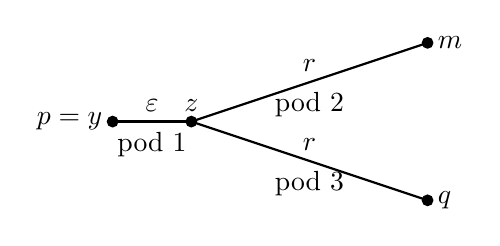
\begin{tikzpicture}[every path/.style={thick}, baseline=(current bounding box.center)]
		\coordinate[label=left:{$p=y$}] (x) at (-1,0); 
		\coordinate[label=above:{$z$}] (m) at (0,0); 
		\coordinate[label=right:{$q$}] (y) at (3,-1); 
		\coordinate[label=right:{$m$}] (z) at (3,1); 
		\draw (x)--(m) node[midway, above] {$\varepsilon$} node[midway, below] {pod 1};
		\draw (y)--(m) node[midway, above] {$r$} node[midway, below] {pod 3};
		\draw (z)--(m) node[midway, above] {$r$} node[midway, below] {pod 2};
		\draw[fill] (x) circle [radius=0.06]; 
		\draw[fill] (m) circle [radius=0.06]; 
		\draw[fill] (y) circle [radius=0.06]; 
		\draw[fill] (z) circle [radius=0.06]; 
	\end{tikzpicture} }
	\caption{Tripod counter-example for the strong quadruple inequality}
	\label{fig:tripod}
	\end{center}
\end{figure}
%
We take $\mf c = d^2$, $\xi=1$, $\mf l = d$, $\mf a = K d$, and $\mf b_m = d_{m}^{\ms{proj}}$.
Then 
\begin{align*}
	\frac{\olc yq - \olc ym - \olc zq + \olc zm}{\mf l(q,m)}
	-
	\frac{\olc yp - \olc ym - \olc zp + \olc zm}{\mf l(p,m)}
	&=
	2 \varepsilon\eqcm
	\\
	\mf a(y,z) \mf b_m(q,p) = K \varepsilon \sqrt{2\frac{\varepsilon}{r+\varepsilon}}
	\eqfs
\end{align*}
If the strong quadruple inequality holds, then
\begin{equation*}
	K  \geq \sqrt{2\frac{r+\varepsilon}{\varepsilon}} \xrightarrow{\varepsilon\searrow0} \infty
	\eqfs
\end{equation*}
Thus, $d_{m}^{\ms{proj}}$ is not a suitable candidate for the strong quadruple distance in general Hadamard spaces.
%
%
%
%
\section{Optimality of Power Inequality}\label{app:power_inequ_opti}
%
We show that $8\alpha2^{-2\alpha}$ is the optimal constant, and that we cannot extend \autoref{thm:power_inequ} to $\alpha > 1$ or $\alpha < \frac12$.
Let $\epsilon\in(0,1)$ and $(\mc Q, d)$ be a metric space with $q,p,y,z\in\mc Q$ such that for each case below the distances have the values written down in \autoref{tbl:dists}. One can easily show that in all three cases the necessary triangle inequalities and the nice quadruple inequality hold.
%
\begin{table}
\begin{center}
\begin{tabular}{c||c|c|c|c|c|c}
	 Case&$\ol yq$ & $\ol yp$ & $\ol zq$ & $\ol zp$ & $\ol yz$ & $\ol qp$  \\ 
	\hline 
	\hline 
	 (a) &$1-\epsilon$ & $1-3\epsilon$ & $1-2\epsilon$ & $1$ & $2-3\epsilon$ & $2\epsilon$\\
	 \hline 
	 (b) & $1$ & $\epsilon$ & $1-\epsilon$ & $2\epsilon$ & $2\epsilon$ & $1$\\
	 \hline 
	 (c) & $2\epsilon$ & $\epsilon$ & $1$ & $1$ & $1$ & $\epsilon$ \\
\end{tabular}
\caption{Distances of four points $y,z,q,p\in\mc Q$ for showing lower bounds of the constant in \autoref{thm:power_inequ}.}
\label{tbl:dists}
\end{center}
\end{table}
%%
%\begin{table}
%	\begin{center}
%		\begin{tabular}{c||c|c|c|c|c}
%			Case&metric space&$y$ & $q$ & $p$ & $z$ \\ 
%			\hline 
%			\hline 
%			(a) & $(\R, |\cdot|)$ & $0$ & $1-3\epsilon$ &  $1-\epsilon$  &  $2-3\epsilon$ \\
%			(b) & $(\R^3, \norm)$ & $(\epsilon/2,\epsilon\sqrt{15}/2,0)$ & $(0,(5\epsilon-2)/\sqrt{15},\sqrt{11/15-2\epsilon/3 -2\epsilon^2/3})$ &  $(-\epsilon/2,\epsilon\sqrt{15}/2,0)$  &  $(0,0,0)$ \\
%		\end{tabular}
%		\caption{Realizations of the distances in \autoref{tbl:dists}.}
%		\label{tbl:value}
%	\end{center}
%\end{table}
%
\begin{enumerate}[label=(\alph*)]
\item 
	For $\alpha \in [\frac12,1]$, we have, using l'Hôpital's rule,
	\begin{align*}
	&\lim_{\epsilon\searrow0}\frac{\ol yq^{2\alpha} - \ol yp^{2\alpha} - \ol zq^{2\alpha} + \ol zp^{2\alpha}}{ \ol yz^{2\alpha-1}\, \ol qp} 
	\\&= 
	\lim_{\epsilon\searrow0}\frac{(1-\epsilon)^{2\alpha} - (1-3\epsilon)^{2\alpha} - (1-2\epsilon)^{2\alpha} + 1}{ (2\epsilon)(2-3\epsilon)^{2\alpha-1}}
	\\&=
	\lim_{\epsilon\searrow0} 2\alpha\frac{-(1-\epsilon)^{2\alpha-1} + 3(1-3\epsilon)^{2\alpha-1} + 2(1-2\epsilon)^{2\alpha-1}}{ 2(2-3\epsilon)^{2\alpha-1}-6\epsilon(2\alpha-1)(2-3\epsilon)^{2\alpha-2}}
	\\&=8\alpha2^{-2\alpha}
	\eqfs
	\end{align*}
	Thus, the constant $8\alpha2^{-2\alpha}$ in \autoref{thm:power_inequ} is optimal.
\item	
	For $\alpha >1$, we have, using l'Hôpital's rule,
	\begin{align*}
	&\lim_{\epsilon\searrow0}\frac{\ol yq^{2\alpha} - \ol yp^{2\alpha} - \ol zq^{2\alpha} + \ol zp^{2\alpha}}{ \ol yz^{2\alpha-1}\, \ol qp} 
	\\&= 
	\lim_{\epsilon\searrow0} \frac{1 -\epsilon^{2\alpha} - (1-\epsilon)^{2\alpha} + (2\epsilon)^{2\alpha}}{ (2\epsilon)^{2\alpha-1}} 
	\\&=
	\frac{2\alpha}{2\alpha-1} \lim_{\epsilon\searrow0} \frac{ - \epsilon^{2\alpha-1} + (1-\epsilon)^{2\alpha-1} + 2	(2\epsilon)^{2\alpha-1}}{ 2^{2\alpha-1}\epsilon^{2\alpha-2}}
	\\&=
	\infty
	\eqfs
	\end{align*}
	Thus, there is no power inequality in the form of \autoref{thm:power_inequ} for $\alpha > 1$.
\item
	For $\alpha \in (0,\frac12)$, we have
	\begin{align*}
	&\lim_{\epsilon\searrow0}\frac{\ol yq^{2\alpha} - \ol yp^{2\alpha} - \ol zq^{2\alpha} + \ol zp^{2\alpha}}{ \ol yz^{2 \alpha-1}\, \ol qp} 
	\\&= 
	\lim_{\epsilon\searrow0}\frac{(2\epsilon)^{2\alpha} - \epsilon^{2\alpha} - 1 + 1}{\epsilon} 
	\\&=
	\lim_{\epsilon\searrow0} (2^{2\alpha}-1)\epsilon^{2\alpha-1}
	\\&=\infty
	\eqfs
	\end{align*}
	Thus, there is no power inequality in the form of \autoref{thm:power_inequ} for $\alpha < \frac12$.
\end{enumerate}
%
%
%
\section{Chaining}\label{app:chaining}
%
Recall the measures of entropy $\gamma_2$ and $\entrn$ defined in \autoref{chaining:def_entropy}. We add another useful entry to this list.
\begin{definition}[Bernoulli Bound]\label{chaining:entropy}
	For $T \subset \R^n$ define
	\begin{equation*}
		b(T) := \inf\cbOf{\sup_{t\in T_1} \normof{t}_1 + \gamma_2(T_2)\,\colon\, T_1, T_2 \subset \R^n, T \subset T_1+T_2}
		\eqcm
	\end{equation*}
	where $\gamma_2(T_2) = \gamma_2(T_2, d_2)$ for the Euclidean metric $d_2$ on $\R^n$, $\normof{t}_1 = \sum_{i=1}^n \abs{t_i}$, and $T_1 + T_2 = \cb{t_1 + t_2 \colon t_1 \in T_1, t_2 \in T_2}$.
\end{definition}
%
We write down the Bernoulli bound for powers of the Bernoulli process. \cite{bednorz14} show that the bound can be reversed (up to an universal constant). Thus, this step can be regarded as optimal.
%
\begin{theorem}[Bernoulli bound]\label{chaining:bernoulli}
	Let $\sigma_1, \dots, \sigma_n$ be independent random signs, i.e., $\Prof{\sigma_i = \pm1} =\frac12$.
	For $t\in R^n$ set $\tilde X_t :=\sum_{i=1}^n \sigma_i t_i$. Let $T \subset \R^n$.
	Let $\kappa \geq 1$.
	Then 
	\begin{equation*}
		\Ex*{\sup_{t\in T} \abs{\tilde X_t}^\kappa} \leq c_\kappa b(T)^\kappa
		\eqcm
	\end{equation*}
	where $c_\kappa$ depends only on $\kappa$.
\end{theorem}
%
\begin{proof}
Let $T_1, T_2 \subset \R^n$ such that $T \subset T_1 + T_2$.
As $(a+b)^\kappa \leq 2^{\kappa-1}\br{a^\kappa + b^\kappa}$ for all $a,b\geq 0$, we can split the supremum into two parts,
\begin{align*}
\Ex*{\sup_{t\in T} \abs{\tilde X_t}^\kappa} 
\leq
2^{\kappa-1} \br{\Ex*{\sup_{t\in T_1} \abs{\tilde X_t}^\kappa}  + \Ex*{\sup_{t\in T_2} \abs{\tilde X_t}^\kappa}}
\eqfs
\end{align*}
The first term is bounded using the 1-norm,
$\Ex*{\sup_{t\in T_1} \abs{\tilde X_t}^\kappa} \leq \sup_{t\in T_1} \normof{t}_1^\kappa$. For the second we use Talagrand's generic chaining bound for the supremum of the subgaussian process $\Ex*{\sup_{t\in T_2} \abs{\tilde X_t}^\kappa} \leq c_\kappa\pr \gamma_2(T_2)^\kappa$, see \cite{talagrand14}. We obtain
\begin{align*}
\Ex*{\sup_{t\in T} \abs{\tilde X_t}^\kappa} 
&\leq 
c_\kappa \br{\sup_{t\in T_1} \normof{t}_1^\kappa + \gamma_2(T_2)^\kappa}
\\&\leq 
c_\kappa \br{\sup_{t\in T_1} \normof{t}_1 + \gamma_2(T_2)}^\kappa
\eqfs
\end{align*}
\end{proof}
%
\begin{lemma}[Lipschitz connection]\label{chaining:lipschitz}
Let $(\mc Q, b)$ be a pseudo-metric space.
Assume there are function $f_i \colon \mc Q \to \R$ such that $\abs{f_i(q) - f_i(p)} \leq a_i b(q,p)$.
Let $T := \cb{(f_i(q))_{i=1,\dots,n} \colon q\in\mc Q}$. Set $a = (a_1, \dots, a_n)$.
Then
\begin{equation*}
	b(T) \leq C \normof{a}_2 \min\brOf{\entrn(\mc Q, b), \gamma_2(\mc Q, b)}
	\eqcm
\end{equation*}
where $C>0$ is an universal constant.
\end{lemma}
%
\begin{proof}
	For $\epsilon>0$, choose $\mc Q_2$ to be an $\epsilon$-covering of $\mc Q$ with respect to $b$, i.e., for all $q \in \mc Q$ there is a $p_q \in \mc Q_2$ such that $b(q,p_q) \leq \epsilon$. For $q\in\mc Q$ denote $t_q := (f_i(q))_{i=1,\dots,n} \in \R^n$. Define $T_2 := \cb{t_p \colon p\in\mc Q_2}$ and $T_1 := \cb{t_q - t_{p_q} \colon q\in Q}$. Then $T \subset T_1 + T_2$.
		The Lipschitz-condition implies $\normof{t_q-t_p}_2 \leq \normof{a}_2 b(q,p)$ for all $q,p\in\mc Q$.
		Thus, 
		\begin{equation*}
			\sup_{t\in T_1} \normof{t}_1 \leq \sup_{q \in \mc Q} \sqrt{n}\normof{t_q-t_{p_q}}_2 \leq \epsilon \sqrt{n} \normof{a}_2 
			\eqfs
		\end{equation*}
		By the properties of $\gamma_2$, see \cite{talagrand14}, we obtain
		\begin{equation*}
			\gamma_2(T_2) \leq c \normof{a}_2 \gamma_2(\mc Q_2, b) \leq c\pr \normof{a}_2  \int_{\epsilon}^\infty \!\! \sqrt{\log N(Q, b, r)} \dl r
		\end{equation*}
		for universal constants $c, c\pr>0$. Applying the two inequalities to the definition of $b(T)$ concludes the proof.
\end{proof}
%
\begin{lemma}[Symmetrization]\label{lmm:symm}
	Let $\mc Q$ be set. Let $Z_1, \dots, Z_n$ be centered, independent, and integrable stochastic processes indexed by $\mc Q$. Let $\Phi\colon \R\to\R$ be a convex, non-decreasing function. Let $(Z_1\pr, \dots, Z_n\pr)$ be an independent copy of $(Z_1, \dots, Z_n)$. Let $\varepsilon_1, \dots, \varepsilon_n$ be iid with $\Prof{\varepsilon_1 = \pm1} = \frac12$.
	Then
	\begin{equation*}
		\Ex*{\sup_{q\in\mc Q} \Phi\brOf{\sum_{i=1}^nZ_i(q)}} \leq
		\Ex*{\sup_{q\in\mc Q} \Phi\brOf{\sum_{i=1}^n\varepsilon_i\br{Z_i(q) - Z_i\pr(q)}}}
		\eqcm
	\end{equation*}
	assuming measurability of the involved terms.
\end{lemma}
%
The symmetrization lemma is well-known. The statement here is an intermediate step of from the proof of \cite[2.3.6 Lemma]{vaart96}.
%
\begin{theorem}[Empirical process bound]\label{chaining:empproc}
	Let $(\mc Q, b)$ be a separable pseudo-metric space. Let $Z_1, \dots, Z_n$ be centered, independent, and integrable stochastic processes indexed by $\mc Q$ with a $q_0 \in \mc Q$ such that $Z_i(q_0) = 0$ for $i=1,\dots, n$.
	Let $(Z_1\pr, \dots, Z_n\pr)$ be an independent copy of $(Z_1, \dots, Z_n)$.
	Assume the following Lipschitz-property: There is a random vector $A$ with values in $\R^n$ such that
	\begin{equation*}
		\abs{Z_i(q)-Z_i(p)-Z_i\pr(q)+ Z_i\pr(p)} \leq A_i b(q,p)
	\end{equation*} 
	for $i = 1,\dots, n$ and all $q,p\in\mc Q$.
	Let $\kappa \geq 1$.
	Then
	\begin{equation*}
		\Ex*{\sup_{q\in\mc Q} \abs{\sum_{i=1}^nZ_i(q)}^\kappa} \leq C_\kappa\, \Ex*{\normof{A}_2^\kappa} \, 
		\min\brOf{\entrn(\mc Q, b), \gamma_2(\mc Q, b)}^\kappa
		\eqcm
	\end{equation*}
	where $C_\kappa > 0$ is a constant depending only on $\kappa$.
\end{theorem}
%
\begin{proof}
	Use \autoref{lmm:symm}. Then apply \autoref{chaining:bernoulli} and \autoref{chaining:lipschitz} conditionally on $Z_1, \dots, Z_n$.
\end{proof}
%
\begin{lemma}\label{lmm:chaining:rate}
Let $(\mc Q, b)$ be a pseudo-metric space.
Let $D >0 $ such that $\diam(\mc Q, b) \leq D < \infty$.
Let $\beta > 0$. Assume 
\begin{equation*}
	\sqrt{\log(N(\mc Q, b , r))} \leq c_{\ms e} \br{\frac{D}{r}}^\beta
\end{equation*}
for all $0 < r < D$.
\begin{enumerate}[label=\environmentEnumerateLabel]
	\item If $\beta < 1$ then $\entrn(\mc Q, b) \leq \frac{c_{\ms e}D}{1-\beta}$.
	\item If $\beta = 1$ then $\entrn(\mc Q, b) \leq c_{\ms e}\pr D \log(n+1)$, where $c\pr>0$ depends only on $c_{\ms e}$.
	\item If $\beta > 1$ then $\entrn(\mc Q, b) \leq c_{\ms e}^{\frac1\beta} \frac\beta{\beta-1} n^{-\frac1{2\beta}+\frac12}$.
\end{enumerate}
In particular
\begin{equation*}
	n^{-\frac12} \,\entrn(\mc Q, b) \ \leq\  c \, D\, \eta_{\beta,n} \eqcm
\end{equation*}
where $c$ depends only on $c_{\ms e}$ and $\beta$ and
\begin{equation*}
	\eta_{\beta,n} := 
	\begin{cases} 
		n^{-\frac12} & \text{ for }\beta < 1\eqcm\\
		n^{-\frac12} \log(n+1) & \text{ for } \beta = 1\eqcm\\
		n^{-\frac1{2\beta}} & \text{ for } \beta > 1\eqfs
	\end{cases} 
\end{equation*}
\end{lemma}
The proof consists of calculating the entropy integral with the given bound on the covering numbers and, for $\beta \geq 1$, choosing the minimizing starting point of the integral $\epsilon>0$.
%
%
%
%
%
%
%
\section{Proof of the Power Inequality, \autoref{thm:power_inequ}}\label{app:power_inequality}
%
%
Let $(\mc Q, d)$ be a metric space. Use the short notation $\ol qp := d(q,p)$.
Let $q,p,y,z\in\mc Q$, $\alpha\in[\frac12,1]$. 
Assume
\begin{equation*}
	\olt yq - \olt yp - \olt zq + \olt zp \leq 2 \, \ol yz\, \ol qp
	\eqfs
\end{equation*}
The goal of this section is to prove 
\begin{equation*}
	\ol yq^{2\alpha} - \ol yp^{2\alpha} - \ol zq^{2\alpha} + \ol zp^{2\alpha} \leq 8 \alpha 2^{-2\alpha} \, \ol yz^{2\alpha-1}\, \ol qp
	\eqfs
\end{equation*}
%
%
%
\subsection{Arithmetic Form}
%
\autoref{thm:power_inequ} will be proven in the form of \autoref{con:ana}. 
%
\begin{lemma}\label{con:ana}
	Let $a,b,c\geq0$, $r,s\in[-1,1]$, and $\alpha\in[\frac12, 1]$.
	Then
	\begin{align*}
		&a^{2\alpha}-c^{2\alpha}-\br{a^2-2rab+b^2}^\alpha+\br{c^2-2scb+b^2}^\alpha 
		\\&\leq 
		8 \alpha 2^{-2\alpha} b \max(ra - sc, |a-c|)^{2\alpha-1}
		\eqfs
	\end{align*}
\end{lemma}
%
The advantage of using \autoref{con:ana} to prove \autoref{thm:power_inequ} is, that we do not need to consider a system of additional conditions for describing that the real values in the inequality are distances, which have to fulfill the triangle inequality. The disadvantage is, that we loose the possibility for a geometric interpretation of the proof.
%
\begin{lemma}\label{lmm:power_implies}
	\autoref{con:ana} implies \autoref{thm:power_inequ}.
\end{lemma}
%
\begin{proof}
	Three points from an arbitrary metric space can be embedded in the Euclidean plane so that the distances are preserved.
	Thus, the cosine formula of Euclidean geometry can be applied to the three points $y,p,q\in\mc Q$: It holds
	\begin{equation*}
		\ol yq^2 = \ol yp^2 + \ol qp^2 - 2 s \,\ol yp\, \ol qp\eqcm
	\end{equation*}
	where $s := \cos(\measuredangle ypq)$ with the angle $\measuredangle ypq$ in the Euclidean plane.
	Similarly
	\begin{equation*}
		\ol zq^2 = \ol zp^2 + \ol qp^2 - 2 r \,\ol zp\, \ol qp
		\eqcm
	\end{equation*}
	where $r := \cos(\measuredangle zpq)$. Thus,
	\begin{align*}
		&
		\ol yq^{2\alpha} - \ol yp^{2\alpha} - \ol zq^{2\alpha} + \ol zp^{2\alpha}
		\\&=
		\br{\ol yp^2 + \ol qp^2 - 2 s \,\ol yp\, \ol qp}^\alpha
		-
		\br{\ol zp^2 + \ol qp^2 - 2 r \,\ol zp\, \ol qp}^\alpha
		- \ol yp^{2\alpha}
		+ \ol zp^{2\alpha}
		\\&=
		\br{c^2 + b^2 - 2 s cb}^\alpha
		-
		\br{a^2 + b^2 - 2 r ab}^\alpha
		- c^{2\alpha}
		+ a^{2\alpha}
		\eqcm
	\end{align*}
	where $a:=\ol zp$, $c:=\ol yp$, $b:=\ol qp$.
	Hence, \autoref{con:ana} yields
	\begin{align}\label{eq:arith:intermediate}
		\ol yq^{2\alpha} - \ol yp^{2\alpha} - \ol zq^{2\alpha} + \ol zp^{2\alpha}
		\leq
		8 \alpha 2^{-2\alpha} b \max(ra - sc, |a-c|)^{2\alpha-1}
		\eqfs
	\end{align}
	The assumption of \autoref{thm:power_inequ} states $\olt yq - \olt yp - \olt zq + \olt zp \leq 2 \, \ol yz\, \ol qp$.
	This implies
	\begin{equation*}
		2b \br{ra-sc}
		=
		\br{c^2 + b^2 - 2 scb}
		-
		\br{a^2 + b^2 - 2 rab}
		- c^{2}
		+ a^{2}
		\leq 
		2 b\,
		\ol yz
		\eqfs
	\end{equation*}
	Therefore, $ra-sc \leq \ol yz$ (or $b=0$, but then $q=p$ and \autoref{thm:power_inequ} becomes trivial).
	Furthermore, the triangle inequality implies $|a-c| = |\ol zp-\ol yp| \leq \ol yz$.
	Thus, we obtain
	\begin{equation}\label{eq:arith:maxbound}
		\max(ra - sc, |a-c|) \leq\ol yz
		\eqfs
	\end{equation}
	Finally, \eqref{eq:arith:intermediate} and \eqref{eq:arith:maxbound} together yield
	\begin{align*}
		\ol yq^{2\alpha} - \ol yp^{2\alpha} - \ol zq^{2\alpha} + \ol zp^{2\alpha}
		\leq
		8 \alpha 2^{-2\alpha}  \,\ol qp\, \ol yz^{2\alpha-1}
		\eqfs
	\end{align*}
\end{proof}
%
The remaining part of this section is dedicated to proving \autoref{con:ana}.

The proof of \autoref{con:ana} can be described as \textit{brute force}. We will distinguish many different cases, i.e., certain bounds on $a,b,c,r,s$, e.g., $a\leq c$ and $a> c$. In each case, we try to simplify the inequality step by step until we can solve it easily. Mostly, the simplification consists of taking some derivative and showing that the derivative is always negative (or always positive). Then we only need to show the inequality at one extremal point. This process may have to be iterated. It is often not clear immediately which derivative to take in order to simplify the inequality. Even after finishing the proof there seems to be no deeper reason for distinguishing the cases that are considered. Thus, unfortunately, the proof does not create a deeper understanding of the result.
%
%
%
\subsection{First Proof Steps and Outline of the Remaining Proof}
%
We want to show \autoref{con:ana} to prove \autoref{thm:power_inequ}.
We refer to the left hand side of the inequality, $a^{2\alpha}-c^{2\alpha}-\br{a^2-2rab+b^2}^\alpha+\br{c^2-2scb+b^2}^\alpha $, as LHS. By RHS we, of course, mean the right hand side, $8 \alpha 2^{-2\alpha} b \max(ra - sc, |a-c|)^{2\alpha-1}$.

For $\max(ra - sc, |a-c|)=0$ we have $a=c$ and $r\leq s$. Thus, LHS $\leq 0$. If $\max(ra - sc, |a-c|)>0$, LHS and RHS are continuous in all parameters. Thus, it is enough to show the inequality on a dense set. In particular, we can and will ignore certain special cases in the following which might introduce technical problems, e.g., "$0^0$".

We have to distinguish the cases $|a-c|=\max(ra - sc, |a-c|)$ and $ra - sc=\max(ra - sc, |a-c|)$. We further distinguish $a\geq c$ and $c \geq a$.
%
\begin{lemma}[$ra - sc$ vs $|a-c|$]\label{lmm:srbound}
	Let $a,b,c\geq0$, $r,s\in[-1,1]$, and $\alpha\in[\frac12, 1]$.
	Then
	\begin{align*}
		&ra - sc \geq a-c
		\quad\Leftrightarrow\quad 
		s 
		\leq
		(r-1) \frac ac+1
		\quad\Leftrightarrow\quad 
		r \geq 
		(s-1)\frac ca +1
		\eqcm
\\
		&ra - sc \geq c-a
		\quad\Leftrightarrow\quad 
		s 
		\leq
		(r+1) \frac ac -1
		\quad\Leftrightarrow\quad 
		r \geq 
		(s+1)\frac ca -1
		\eqfs
	\end{align*}
\end{lemma}
\begin{proof}
It holds
	\begin{align*}
	&
		ra - sc \geq a-c
		\quad\Leftrightarrow\quad
		ra - a+c \geq sc
		\quad\Leftrightarrow\quad
		\frac{a(r-1)+c}{c} \geq s
\eqcm\\&
		ra - sc \geq c-a
		\quad\Leftrightarrow\quad
		ra - c+a \geq sc
		\quad\Leftrightarrow\quad
		\frac{a(r+1)-c}{c} \geq s
\eqcm\\&
		ra - sc \geq a-c
	\quad	\Leftrightarrow\quad
		ra \geq a-c+sc
		\quad\Leftrightarrow\quad
		r \geq (s-1)\frac ca +1
\eqcm\\&
		ra - sc \geq c-a
		\quad\Leftrightarrow\quad
		ra  \geq c-a+sc
		\quad\Leftrightarrow\quad
		r \geq (s+1)\frac ca -1
\eqfs
	\end{align*}
\end{proof}
%
%
%
%
\subsubsection{The Case $|a-c| \leq ra-sc$}
%
Consider the case $ra-sc \geq |a-c|$. The next lemma shows convexity in $r$ of the function "LHS minus RHS". This means, we only have to check values of $r$ on the border of its domain.
%
\begin{lemma}[Convexity in $r$]\label{lmm:ddr}
	Let $a,b,c\geq0$, $s,r\in[-1,1]$, $\alpha\in[\frac12,1]$.
	Assume $ra - sc \geq 0$.
	Define 
	\begin{align*}
		F(r,s) 
		:= 
		&\,a^{2\alpha}-c^{2\alpha}-\br{a^2-2rab+b^2}^\alpha+\br{c^2-2scb+b^2}^\alpha 
		\\&-
		8 \alpha 2^{-2\alpha} b (ra - sc)^{2\alpha-1}
		\eqfs
	\end{align*}
	Then
	\begin{equation*}
		\partial_r^2 F(r,s) \geq 0
		\eqfs
	\end{equation*}
\end{lemma}
%
Note, neither $\partial_s^2 F(r,s) \geq 0$ nor $\partial_s^2 F(r,s) \leq 0$ for all $a,b,c,s,r$.
%
\begin{proof}
	Define
	\begin{equation*}
		\ell(r,s) := a^{2\alpha}-c^{2\alpha}-\br{a^2-2rab+b^2}^\alpha+\br{c^2-2scb+b^2}^\alpha 
		\eqfs
	\end{equation*}
	It holds
	\begin{align*}
		\partial_r \ell(r,s) &= 2ab\alpha\br{a^2-2rab+b^2}^{\alpha-1}\eqfs
	\end{align*}
	Define $h(r,s) := 8 \alpha 2^{-2\alpha} b \br{ra - sc}^{2\alpha-1}$. It holds
	\begin{align*}
		\partial_r h(r,s) &= 8 \alpha (2\alpha-1) 2^{-2\alpha} b a \br{ra - sc}^{2\alpha-2}\eqfs
	\end{align*}
	It holds $F(r,s) = \ell(r,s)-h(r,s)$.
	It holds
	\begin{align*}
		f(r) :=	 \frac{	\partial_r \ell(r,s)-\partial_r h(r,s)}{2ab\alpha} &= \br{a^2-2rab+b^2}^{\alpha-1} - (2\alpha-1) \br{\frac{ra - sc}{2}}^{2\alpha-2}
	\end{align*}
	and 
	\begin{align*}
		\partial_r f(r) 
		&= 
		-2ab(\alpha-1) \br{a^2-2rab+b^2}^{\alpha-2} 
		- \frac12 a(2\alpha-1)(2\alpha-2) \br{\frac{ra - sc}{2}}^{2\alpha-3} 
		\eqfs
	\end{align*}
	It holds $2ab \br{a^2-2rab+b^2}^{\alpha-2} \geq 0$ and $(\alpha-1) \leq 0$. Thus,
	\begin{equation*}
		-2ab(\alpha-1) \br{a^2-2rab+b^2}^{\alpha-2} \geq 0\eqfs
	\end{equation*}
	It holds $\frac12 a(2\alpha-1) \br{\frac{ra - sc}{2}}^{2\alpha-3} \geq 0$ and  $(2\alpha-2)\leq 0$. Thus, $-\frac12 a(2\alpha-1)(2\alpha-2) \br{\frac{ra - sc}{2}}^{2\alpha-3} \geq 0$. Hence,	$\partial_r f(r) \geq 0$. Hence, $\partial_r^2 F(r,s) \geq 0$.
\end{proof}
%
%
%
%
%
\subsubsection{The Case $|a-c| \geq ra-sc$}\label{ssec:acgreasc}
%
In the case $|a-c| \geq ra-sc$, the RHS does not depend on $s$ or $r$. Thus, we maximize the LHS with respect to $r$ and $s$ and only need to show the inequality for this maximized term.

Define
\begin{equation*}
	\ell(r,s) := a^{2\alpha}-c^{2\alpha}-\br{a^2-2rab+b^2}^\alpha+\br{c^2-2scb+b^2}^\alpha 
	\eqfs
\end{equation*}
It holds
\begin{equation*}
	\max_{s\geq s_0, r\leq r_0} \ell(r,s) = \ell(r_0,s_0)
	\eqfs
\end{equation*}
Distinguish the two cases $a\geq c$ and $a\leq c$.\\
\underline{Case 1: $a\geq c$.} For fixed $r\in[-1,1]$, set $s = s_{\ms{min}}(r) = (r-1) \frac ac+1$, cf \autoref{lmm:srbound}. Define
\begin{align*}
	f(r) &:= \ell(r,s_{\ms{min}}(r)) 
	\\&= a^{2\alpha}-c^{2\alpha}-\br{a^2-2rab+b^2}^\alpha+\br{c^2-2rab+2ab-2cb+b^2}^\alpha
	\eqfs
\end{align*}
Then
\begin{equation*}
	\frac{f\pr(r)}{2ab\alpha} = \br{a^2-2rab+b^2}^{\alpha-1} - \br{c^2-2rab+2ab-2cb+b^2}^{\alpha-1}
	\eqfs
\end{equation*}
\underline{Case 1.1: $a^2 \leq c^2+2ab-2cb$.} Then
\begin{align*}
	a^2-2rab+b^2 &\leq c^2-2rab+2ab-2cb+b^2\eqcm\\
	\br{a^2-2rab+b^2}^{\alpha-1} &\geq \br{c^2-2rab+2ab-2cb+b^2}^{\alpha-1}
	\eqfs
\end{align*}
Thus, $f\pr(r)\geq0$. In this case, we need to show
\begin{equation*}
	a^{2\alpha}-c^{2\alpha}-|a-b|^{2\alpha}+|c-b|^{2\alpha} = f(1) \leq 8\alpha 2^{-2\alpha} b (a-c)^{2\alpha-1}
	\eqfs
\end{equation*}
\underline{Case 1.2: $a^2 \geq c^2+2ab-2cb$.} Then
\begin{align*}
	a^2-2rab+b^2 &\geq c^2-2rab+2ab-2cb+b^2\eqcm\\
	\br{a^2-2rab+b^2}^{\alpha-1} &\leq \br{c^2-2rab+2ab-2cb+b^2}^{\alpha-1}\eqfs
\end{align*}
Thus, $f\pr(r)\leq0$. The relevant values are $r = r_{\ms{min}} = 1-2\frac ca$, with $s = s_{\ms{min}}(r) = -1$. In this case, we need to show
\begin{equation*}
	a^{2\alpha}-c^{2\alpha}-\br{(a-b)^2+4cb}^{\alpha}+(c+b)^{2\alpha} = f(r_{\ms{min}}) \leq 8\alpha 2^{-2\alpha} b (a-c)^{2\alpha-1}
	\eqfs
\end{equation*}
\underline{Case 2: $a\leq c$.}  For fixed $r\in[-1,1]$, set $s = s_{\ms{min}}(r) = (r+1) \frac ac-1$. Define
\begin{align*}
	f(r) &:= \ell(r,s_{\ms{min}}(r)) 
	\\&= a^{2\alpha}-c^{2\alpha}-\br{a^2-2rab+b^2}^\alpha+\br{c^2-2rab-2ab+2cb+b^2}^\alpha
	\eqfs
\end{align*}
Then 
\begin{equation*}
	\frac{f\pr(r)}{2ab\alpha} = 
	\br{a^2-2rab+b^2}^{\alpha-1} - \br{c^2-2rab-2ab+2cb+b^2}^{\alpha-1}
	\eqfs
\end{equation*}
\underline{Case 2.1: $a^2 \leq c^2-2ab+2cb$.} Then
\begin{align*}
	a^2-2rab+b^2 &\leq c^2-2rab-2ab+2cb+b^2\eqcm\\
	\br{a^2-2rab+b^2}^{\alpha-1} &\geq \br{c^2-2rab-2ab+2cb+b^2}^{\alpha-1}\eqfs
\end{align*}
Thus, $f\pr(r)\geq0$. The critical value is $r = r_{\ms{max}} = 1$, with $s = s_{\ms{min}}(r) = 2\frac ac-1$. In this case, we need to show
\begin{equation*}
	a^{2\alpha}-c^{2\alpha}-|a-b|^{2\alpha}+\br{(c+b)^2-4ab}^{\alpha} = f(1) \leq 8\alpha 2^{-2\alpha} b (c-a)^{2\alpha-1}
	\eqfs
\end{equation*}
\underline{Case 2.2: $a^2 \geq c^2-2ab+2cb$.} This cannot happen for $a\leq c$.
%
\begin{remark}
Assume $a\geq c$. Then
\begin{align*}
	a^2 \geq c^2+2ab-2cb
	\quad\Leftrightarrow\quad
	a^2-c^2 \geq 2b(a-c)
	\quad\Leftrightarrow\quad
	a+c \geq 2b
	\eqfs
\end{align*}
\end{remark}
%
%
\subsubsection{Outline}
%
\begin{remark}[What we need to show]\label{rmk:outline}
	Define
	\begin{align*}
		F(r,s) 
		:= 
		&a^{2\alpha}-c^{2\alpha}-\br{a^2-2rab+b^2}^\alpha+\br{c^2-2scb+b^2}^\alpha 
		\\&-
		8 \alpha 2^{-2\alpha} b (ra - sc)^{2\alpha-1}
		\eqfs
	\end{align*}
	\begin{enumerate}[label=(\roman*)]
	\item 
		For the case $a\geq c$, we need $F(1,s) \leq 0$ for all $s\in[-1,1]$ (cf \autoref{lmm:ddr}, includes  case 1.1 of section \ref{ssec:acgreasc}) and $F(1-2\frac ca, -1) \leq 0$ (case 1.2 of section \ref{ssec:acgreasc}).
		Note $r= 1-2\frac ca, s=-1$ means $ra-sc = a-c$.
	\item	
		For the case $a \leq c$, we need $F(1,s) \leq 0$ for all $s\in[-1,2\frac ac-1]$  (cf \autoref{lmm:ddr}, includes case 2.1 of section \ref{ssec:acgreasc}).
		Note $r= 1, s=2\frac ac-1$ means $ra-sc = c-a$.
	\end{enumerate}
	The part $F(1-2\frac ca, -1) \leq 0$ for $a\geq c$ is discussed in section \ref{ssec:rascleqac}.
	The different case for $F(1,s) \leq 0$ ($a\leq c$ and $a\geq c$) are covered in the following way:
	\begin{enumerate}[label=(\alph*)]
	\item 
	$b \geq 2sc$: \autoref{lmm:rascMergingLemma} (Merging Lemma) + \autoref{lmm:tightpowerbound} (Tight Power Bound)
	\item
	$b \leq 2sc$ and $sc \leq a-b$: \autoref{lmm:merging:asc} (Merging Lemma) + \autoref{lmm:tightpowerbound} (Tight Power Bound)
	\item
	$b \leq 2sc$ and $sc \geq a-b$ and $a \geq c$: \autoref{lmm:rascgeqacandageqc} 
	\item 
	$b \leq 2sc$ and $sc \geq a-b$ and $a \leq c$, $sc \leq 2a-c$ and $b \leq 2a-2sc$: \autoref{lmm:bleqasc}
	\item
	$b \leq 2sc$ and $sc \geq a-b$ and $a \leq c$, $sc \leq 2a-c$ and $b \geq 2a-2sc$ and $a \leq b$ : \autoref{lmm:bgeqascandaleqb}
	\item
	$b \leq 2sc$ and $sc \geq a-b$ and $a \leq c$, $sc \leq 2a-c$ and $b \geq 2a-2sc$ and $a \geq b$ : \autoref{lmm:bgeqascandageqb}
	\end{enumerate}
\end{remark}
%
The proofs consist of distinguishing many different cases and applying simple analysis methods in each case.
Nonetheless, finding the poofs is often quite hard, as the inequalities are usually very tight and the right steps necessary for the proof are hard to guess. 

As intermediate steps we can, in some cases, use two lemmas: the Tight Power Bound, see section \ref{ssec:tightpowerbound}, and the Merging Lemma, see \ref{ssec:merginglemma}.
The remaining cases that cannot be solved via Tight Power Bound and Merging Lemma will be discussed in sections \ref{ssec:rascgeqac} and \ref{ssec:rascleqac}.
%
%
%
\subsection{Tight Power Bound}\label{ssec:tightpowerbound}
%
Following lemma gives one very useful inequality in three different forms. It gives a hint to why the power $\dots^{2\alpha-1}$ comes up in the RHS of \autoref{con:ana}.
%
\begin{lemma}[Tight Power Bound]\label{lmm:tightpowerbound}
	Let $x,y\geq0$.
	\begin{enumerate}[label=\environmentEnumerateLabel]
	\item 
		If  $a\in[1,2]$, $x\geq y$, then
		\begin{equation*}
			2^a x^{a-1}y \quad\leq\quad (x+y)^a-(x-y)^a \quad\leq\quad 2a x^{a-1}y \eqfs
		\end{equation*}
	\item 
		If  $a\in[1,2]$, then
		\begin{equation*}
			(x+y)^a-|x-y|^a \quad\leq\quad 2a\min(xy^{a-1},x^{a-1}y)\eqfs
		\end{equation*}
	\item 
		If  $a\in[1,2]$, $x\geq y$, then
		\begin{equation*}
			(x+y)^{a-1} (x-y) \quad\leq\quad x^a - y^a \quad\leq\quad a (x-y) \br{\frac{x+y}{2}}^{a-1}
			\eqfs
		\end{equation*}
	\end{enumerate}
\end{lemma}
%
Note that this result is slightly stronger than the application of the mean value theorem to the function $x \mapsto x^a$, which yields $x^a - y^a \leq a (x-y) z^{a-1}$ for all $x \geq y \geq 0$ and $a > 0$, where $z \in [y,x]$.
%
\begin{proof}
	Assume $x\geq y$.
	Set $z = \frac yx \in[0,1]$. Define
	\begin{equation*}
		f(z) = \frac{(1+z)^a-(1-z)^a}{z}
		\eqfs
	\end{equation*}
	If we can show $f(z) \leq 2a$, then
	\begin{align*}
		&&(1+z)^a-(1-z)^a &\leq 2a z\\
		\Rightarrow && (x+zx)^a-(x-zx)^a &\leq 2a x^a z\\
		\Rightarrow && (x+y)^a-(x-y)^a &\leq 2a x^{a-1} y
		\eqfs
	\end{align*}
	It holds 
	\begin{equation*}
		f\pr(z) = \frac {g(z)}{z^2}
		\eqcm
	\end{equation*}
	where
	\begin{equation*}
		g(z) = az \br{(1+z)^{a-1}+(1-z)^{a-1}}-\br{(1+z)^{a}-(1-z)^{a}}
		\eqfs
	\end{equation*}
	It holds
	\begin{equation*}
		g\pr(z) = az(a-1)\br{(1+z)^{a-2}-(1-z)^{a-2}} \leq 0\eqfs
	\end{equation*}
	Thus, $g(z)\leq g(0) = 0$.
	Thus, $f\pr(z)\leq0$.
	Thus, for all $z_0 \in [0,1]$,
	\begin{equation*}
		f(z_0) 
		\leq 
		\lim_{z\searrow 0}f(z) 
		\stackrel{\ms{L'H}}{=} 
		\lim_{z\searrow 0}\frac{a(1+z)^{a-1}+a(1-z)^{a-1}}{1} 
		= 
		2a
		\eqcm
	\end{equation*}
	where $\ms{L'H}$ indicates the use of L'Hospital's rule. 
	Furthermore, $f(z_0) \geq f(1) = 2^a$, which implies the lower bound. 
	This finishes the proof for (i). The other parts follow immediately.
\end{proof}
%
%
%
\subsection{Merging Lemma}\label{ssec:merginglemma}
%
In many cases (i.e., with additional assumption on $a,b,c,r$ or $s$), we prove the inequality of \autoref{con:ana} by applying first a merging lemma to the LHS to reduce the four summands to two summands of a specific form. Then we apply the Tight Power Bound. The Merging Lemma is discussed in this section.
%
\subsubsection{Simple Merging Lemma}
%
\begin{lemma}[Simple Merging Lemma]\label{lmm:merging:simple}
	Let $\alpha\in[\frac12,1]$, $b\geq0$, $a,c\in\R$.
	Then
	\begin{equation*}
		|a|^{2\alpha}-|c|^{2\alpha}-|a-b|^{2\alpha}+|c-b|^{2\alpha} \leq 
		2^{1-2\alpha} \bigg(
							(a-c + b)^{2\alpha}  -  |a-c - b|^{2\alpha}
						\bigg) \indOf{a-c>0}
		\eqfs
	\end{equation*}
\end{lemma}
%
\begin{proof}
	For $\tilde \alpha\geq 1$, the function $\R\to\R,\, x\mapsto |x|^{\tilde\alpha}-|x-1|^{\tilde\alpha}$ is increasing.
	It holds $2\alpha\geq1$. Thus, if $a\leq c$, then
	\begin{equation*}
		|a|^{2\alpha}-|a-b|^{2\alpha}\leq |c|^{2\alpha}-|c-b|^{2\alpha} 
		\eqfs
	\end{equation*}
	This shows the inequality for the case $a\leq c$.
	
	Set $q:= a-b$ and define
	\begin{equation*}
		g(b) :=  |q+b|^{2\alpha}-|c|^{2\alpha}-|q|^{2\alpha}+|c-b|^{2\alpha} - 2\br{\br{\frac{q-c}{2}+b}^{2\alpha}-\br{\frac{q-c}{2}}^{2\alpha}}
		\eqfs
	\end{equation*}
	It holds $g(0)=0$
	and
	\begin{equation*}
		\frac{g\pr(b)}{2\alpha} = \sgn(q+b)|q+b|^{2\alpha-1}-\sgn(c-b)|c-b|^{2\alpha-1} -
						2\br{\frac{q-c}{2}+b}^{2\alpha-1}
		\eqfs
	\end{equation*}
	\underline{Case 1: $\sgn(q+b) = +1$, $\sgn(c-b)=+1$}:
		\begin{equation*}
			\frac{g\pr(b)}{2\alpha} = (q+b)^{2\alpha-1}-(c-b)^{2\alpha-1} -
							2\br{\frac{q-c}{2}+b}^{2\alpha-1}
			\eqcm
		\end{equation*}
		\begin{equation*}
			(q+b)^{2\alpha-1}-(c-b)^{2\alpha-1} \leq \br{q+b-(c-b)}^{2\alpha-1}\leq 2\br{\frac{q-c}{2}+b}^{2\alpha-1}
			\eqfs
		\end{equation*}
	\underline{Case 2: $\sgn(q+b) = -1$, $\sgn(c-b)=-1$}:
		\begin{equation*}
			\frac{g\pr(b)}{2\alpha} = (b-c)^{2\alpha-1}-(-q-b)^{2\alpha-1}
							-2\br{\frac{q-c}{2}+b}^{2\alpha-1}
			\eqcm
		\end{equation*}
		\begin{equation*}
			(b-c)^{2\alpha-1}-(-q-b)^{2\alpha-1} \leq \br{b-c-(-q-b)}^{2\alpha-1}\leq 2\br{\frac{q-c}{2}+b}^{2\alpha-1}
			\eqfs
		\end{equation*}
	\underline{Case 3: $\sgn(q+b) = +1$, $\sgn(c-b)=-1$}:
		\begin{equation*}
			\frac{g\pr(b)}{2\alpha} = (q+b)^{2\alpha-1}+(b-c)^{2\alpha-1} -
									2\br{\frac{q-c}{2}+b}^{2\alpha-1}
									\eqcm
		\end{equation*}
		\begin{equation*}
			(q+b)^{2\alpha-1}+(b-c)^{2\alpha-1} \leq 2\br{\frac{q-c}{2}+b}^{2\alpha-1}
			\eqfs
		\end{equation*}
	\underline{Case 4: $\sgn(q+b) = -1$, $\sgn(c-b)=+1$}:
		\begin{equation*}
			\frac{g\pr(b)}{2\alpha} = -(-q-b)^{2\alpha-1}-(c-b)^{2\alpha-1} -
									2\br{\frac{q-c}{2}+b}^{2\alpha-1}
									\eqcm
		\end{equation*}
		\begin{equation*}
			-(-q-b)^{2\alpha-1}-(c-b)^{2\alpha-1} \leq 0
			\eqfs
		\end{equation*}
	\underline{Together:}
	In every case, we have $g\pr(b) \leq 0$ and $g(0)=0$. Thus, $g(b) \leq 0$.
\end{proof}
%
%
%
\subsubsection{$ra-sc$--Merging Lemma}
%
\begin{lemma}
	Let $\alpha\in[0,1]$.
	\theoremContentInNewLine
	\begin{enumerate}[label=\environmentEnumerateLabel]
	\item 
		Let $b,c\geq0$, $s\in[-1,1]$.
		Assume $2sc \leq b$.
		Then
		\begin{equation*}
			-c^{2\alpha}+(c^2 - 2 s c b+b^2)^\alpha \leq 
			-|sc|^{2\alpha}+|sc-b|^{2\alpha}
			\eqfs
		\end{equation*}
	\item
		Let $a,b\geq0$, $r\in[-1,1]$.
		Assume $2ra \geq b$.
		Then
		\begin{equation*}
			a^{2\alpha}-(a^2 - 2 r a b+b^2)^\alpha \leq 
			|ra|^{2\alpha}-|ra-b|^{2\alpha}
			\eqfs
		\end{equation*}
	\end{enumerate}
\end{lemma}
%
\begin{proof}
	The function $t \mapsto (t+1)^\alpha-t^\alpha$, $t\geq0$ is non-increasing for all $\alpha\in[0,1]$.
	It holds $0\leq s^2c^2\leq c^2$ and $x := -2 s c b+b^2 \geq 0$. Thus,
	\begin{equation*}
		\br{c^2+x}^\alpha-\br{c^2}^\alpha \leq \br{(sc)^2+x}^\alpha-\br{(sc)^2}^\alpha
		\eqfs
	\end{equation*}
	Thus, 
	\begin{equation*}
		(c^2-2 s c b+b^2)^\alpha -c^{2\alpha}\leq |-sc+b|^{2\alpha}-|sc|^{2\alpha}
		\eqfs
	\end{equation*}
	For the second part, set $x:=2rab-b^2$, $y := a^2-x\geq0$, $\tilde y := |ra|^2-x\geq 0$. The condition $2ra\geq b$ implies $x\geq 0$.
	Thus, as before,
	\begin{equation*}
		a^{2\alpha}-(a^2 - 2 r a b+b^2)^\alpha 
		=
		(y+x)^\alpha-y^\alpha 
		\leq 
		(\tilde y+x)^\alpha-\tilde y^\alpha 
		=
		|ra|^{2\alpha}-|ra-b|^{2\alpha}
		\eqfs
	\end{equation*}
\end{proof}
%
\begin{lemma}[$ra-sc$--Merging Lemma]\label{lmm:rascMergingLemma}
	Let $\alpha\in[\frac12,1]$.
	Let $a,b,c\geq0$, $r,s\in[-1,1]$.
	\theoremContentInNewLine
	\begin{enumerate}[label=\environmentEnumerateLabel]
	\item 
		Assume $2ra \geq b$, $s\in\cb{-1,1}$.
		Then
		\begin{align*}
			&a^{2\alpha}-c^{2\alpha}-(a^2-2rab+b^2)^{\alpha} + (c^2 - 2 s c b + b^2)^\alpha
			\\& \leq 2^{1-2\alpha} \bigg((ra - s c + b)^{2\alpha}-\abs{ra - s c - b}^{2\alpha}\bigg) \ind_{ra-sc>0}
			\eqfs
		\end{align*}	
	\item 
		Assume $b \geq 2sc$, $r\in\cb{-1,1}$.
		Then
		\begin{align*}
			&a^{2\alpha}-c^{2\alpha}-(a^2-2rab+b^2)^{\alpha} + (c^2 - 2 s c b + b^2)^\alpha 
			\\&\leq 2^{1-2\alpha} \bigg((ra - s c + b)^{2\alpha}-\abs{ra - s c - b}^{2\alpha}\bigg)\ind_{ra-sc>0}
			\eqfs
		\end{align*}	
	\item 
		Assume $2ra \geq b \geq 2sc$.
		Then
		\begin{align*}
			&a^{2\alpha}-c^{2\alpha}-(a^2-2rab+b^2)^{\alpha} + (c^2 - 2 s c b + b^2)^\alpha 
			\\&\leq 2^{1-2\alpha} \br{(ra - s c + b)^{2\alpha}-\abs{ra - s c - b}^{2\alpha}}\ind_{ra-sc>0}
			\eqfs
		\end{align*}	
	\end{enumerate}
\end{lemma}
%
\begin{proof}
	The lemma above and the simple merging lemma imply
	\begin{align*} 
		&a^{2\alpha}-c^{2\alpha}-(a^2-2rab+b^2)^{\alpha} + (c^2 - 2 s c b + b^2)^\alpha 
		\\&\leq 
		(ra)^{2\alpha}-(sc)^{2\alpha}-(ra-b)^{2\alpha} + (sc-b)^{2\alpha}
		\\&\leq 
		2^{1-2\alpha} \br{(ra - s c + b)^{2\alpha}-\abs{ra - s c - b}^{2\alpha}}\ind_{ra-sc>0}
		\eqfs
	\end{align*}	
\end{proof}
%
%\begin{lemma}
%	Let $\alpha\in[0,1]$.
%	\theoremContentInNewLine
%	\begin{enumerate}[label=\environmentEnumerateLabel]
%	\item 
%		Let $b,c\geq0$, $s\in[-1,1]$.
%		Then
%		\begin{equation*}
%			(c^2 - 2 s c b+b^2)^\alpha \leq 
%			(c+b)^{2\alpha}
%			\eqfs
%		\end{equation*}
%	\item
%		Let $a,b\geq0$, $r\in[-1,1]$.
%		Then
%		\begin{equation*}
%			-(a^2 - 2 r a b+b^2)^\alpha \leq 
%			-|a-b|^{2\alpha}
%			\eqfs
%		\end{equation*}
%	\end{enumerate}
%\end{lemma}
%%
%\begin{proof}
%	easy
%\end{proof}
%%
%\begin{lemma}[$a+c$--Merging Lemma]
%	Let $\alpha\in[\frac12,1]$.
%	Let $a,b,c\geq0$, $r,s\in[-1,1]$.
%	\theoremContentInNewLine
%	\begin{enumerate}[label=\environmentEnumerateLabel]
%	\item 
%		Then
%		\begin{equation*}
%			a^{2\alpha}-c^{2\alpha}-(a^2-2rab+b^2)^{\alpha} + (c^2 - 2 s c b + b^2)^\alpha \leq 
%			a^{2\alpha}-c^{2\alpha}-|a-b|^{2\alpha} + (c^2 - 2 s c b + b^2)^\alpha 
%			\eqfs
%		\end{equation*}
%	\item
%		Then
%		\begin{equation*}
%			a^{2\alpha}-c^{2\alpha}-(a^2-2rab+b^2)^{\alpha} + (c^2 - 2 s c b + b^2)^\alpha \leq 2^{1-2\alpha} \bigg((a + c + b)^{2\alpha}-\abs{a + c - b}^{2\alpha}\bigg)
%			\eqfs
%		\end{equation*}	
%	\end{enumerate}
%	
%\end{lemma}
%%
%\begin{proof}
%	Merging Lemma and lemma above.
%\end{proof}
%
%
%
\subsubsection{$a-sc$--Merging Lemma}
%
\autoref{lmm:rascMergingLemma} covers the case $\frac12 b \geq sc$.
The following lemma covers  $\frac12 b \leq sc$  under the additional restriction $sc \leq a-b$.
%
\begin{lemma}[$a-sc$--Merging Lemma]\label{lmm:merging:asc}
	Let $\alpha\in[\frac12,1]$.
	Let $a,b,c\geq0$, $s\in[-1,1]$.
	Assume $\frac12 b \leq sc\leq a-b$.
	Then
	\begin{equation*}
		a^{2\alpha}-c^{2\alpha}-(a-b)^{2\alpha}+(c^2 - 2 s c b + b^2)^\alpha \leq 2^{1-2\alpha} \bigg(
			(a - s c + b)^{2\alpha}  -  (a - s c - b)^{2\alpha}
		\bigg)
		\eqfs
	\end{equation*}
\end{lemma}
%
\begin{proof}
	Set $\delta:=a-b$.
	Define
	\begin{align*}
		f(\delta) 
		= &\,(\delta+b)^{2\alpha}-c^{2\alpha}-\delta^{2\alpha}+(c^2 - 2 s c b + b^2)^\alpha -
		\\&2 \br{
					\br{\frac{\delta - s c}{2} + b}^{2\alpha}  -  \br{\frac{\delta - s c}{2}}^{2\alpha}
				}
		\eqfs
	\end{align*}
	Then
	\begin{equation*}
		\frac{f\pr(\delta)}{2\alpha} =
		(\delta+b)^{2\alpha-1}-\delta^{2\alpha-1} 
		- \br{\frac{\delta - s c}{2} + b}^{2\alpha-1}
		+ \br{\frac{\delta - s c}{2}}^{2\alpha-1}
		\eqfs
	\end{equation*}
	It holds
	\begin{align*}
		\delta+b &\geq  \delta\eqcm\\
		\frac{\delta - s c}{2} &\leq  \frac{\delta - s c}{2} + b\eqcm\\
		(\delta+b) + \frac{\delta - s c}{2} &= \delta +\br{\frac{\delta - s c}{2} + b}\eqfs
	\end{align*}
	Thus,
	\begin{equation*}
		(\delta+b)^{2\alpha-1}
		+ \br{\frac{\delta - s c}{2}}^{2\alpha-1}
		\leq
		\delta^{2\alpha-1} 
		+\br{\frac{\delta - s c}{2} + b}^{2\alpha-1}
		\eqfs
	\end{equation*}
	Thus, $f\pr(\delta) \leq 0$.\\ 
	The next lemma shows $f(sc) \leq 0$. Thus, $f(\delta) \leq 0$ for all $\delta \geq sc$.
\end{proof}
%
\begin{lemma}
	Let $x,a,b,c \geq 0$.
	Assume $b \leq 2x$, $x+b \geq c$, $x\leq c$.
	Then
	\begin{equation*}
		(x+b)^{2\alpha}+(c^2 - 2 x b + b^2)^\alpha \leq c^{2\alpha}+x^{2\alpha} + 2 b^{2\alpha} 
		\eqfs
	\end{equation*}	
\end{lemma}
%
\begin{proof}
	Define
	\begin{align*}
		g(x) &:=(x+b)^{2\alpha}+(c^2 - 2 x b + b^2)^\alpha - c^{2\alpha}-x^{2\alpha} - 2 b^{2\alpha} \eqcm
		\\
		h(x) &:= \frac{g\pr(x)}{2\alpha}
		=
		(x+b)^{2\alpha-1}-x^{2\alpha-1}-b(c^2 - 2 x b + b^2)^{\alpha -1}
		\eqfs
	\end{align*}
	It holds
	\begin{equation*}
		h\pr(x)
		=
		(2\alpha-1)(x+b)^{2\alpha-2}-(2\alpha-1)x^{2\alpha-2}+2(\alpha -1) b^2(c^2 - 2 x b + b^2)^{\alpha -2}
		\eqfs
	\end{equation*}
	As $2\alpha-2 \leq 0$ and $2\alpha-1 \geq 0, (2\alpha-1)(x+b)^{2\alpha-2}-(2\alpha-1)x^{2\alpha-2}\leq 0$.
	As $\alpha-1\leq0$, $2(\alpha -1) b^2(c^2 - 2 x b + b^2)^{\alpha -2} \leq 0$.
	Thus, $h\pr(x)\leq0$. \\
	It holds $x\geq x_{\ms{min}} := \max(\frac b2, c-b)$. For checking $h(x_{\ms{min}}) \leq 0$ and $g(x_{\ms{min}}) \leq 0$, we distinguish $x_{\ms{min}} = c-b$ and $x_{\ms{min}} = \frac b2$.\\
	\underline{Case 1, $c-b\leq\frac b2$:}\\
	If $c-b\leq\frac b2$, then $c\leq \frac32 b \leq (1+\sqrt{3})b$, $c^2 -2cb-2b^2\leq0$, and
	\begin{align*}
		h\brOf{c-b} 
		&= 
		c^{2\alpha-1}-(c-b)^{2\alpha-1}-b(c^2 - 2 (c-b) b + b^2)^{\alpha -1}
		\\&= 
		c^{2\alpha-1}-(c-b)^{2\alpha-1}-b(c^2 - 2 c b - b^2)^{\alpha -1}
		\\&\leq 
		b^{2\alpha-1}-b(c^2 - 2 c b - b^2)^{\alpha -1}
		\\&\leq 
		b \br{\br{b^2}^{\alpha-1}-\br{c^2 - 2 c b - b^2}^{\alpha -1}}
	\end{align*}
	And, thus, $h\brOf{c-b}  \leq 0$ as $c^2 -2cb-2b^2\leq0$.
	Furthermore,
	\begin{align*}
		g\brOf{c-b} 
		&=
		-(c-b)^{2\alpha}+(c^2 - 2 c b-b^2)^\alpha 
		- 2 b^{2\alpha} 
		\\&=
		-(c-b)^{2\alpha}+(c^2 - 2 c b-2b^2+b^2)^\alpha 
				- 2 b^{2\alpha} 
		\\&\leq 
		-(c-b)^{2\alpha}+b^{2\alpha }
		- 2 b^{2\alpha} 
		\\&=
		-(c-b)^{2\alpha}
		- b^{2\alpha} 
		\\&\leq
		0
		\eqfs
	\end{align*}
	Thus, $g(x)\leq 0$ for all valid $x$.\\
	\underline{Case 2, $c-b\geq\frac b2$:}\\
	If $c-b\geq\frac b2$, then $c\geq b$ and
	\begin{align*}
		h\brOf{\frac b2} 
		&= 
		\br{\frac32 b}^{2\alpha-1}-\br{\frac12 b}^{2\alpha-1}-b(c^2)^{\alpha -1}
		\\&=
		\br{\br{\frac32}^{2\alpha-1}-\br{\frac12}^{2\alpha-1}} b^{2\alpha-1}-b(c^2)^{\alpha -1}
		\\&\leq 
		b^{2\alpha-1}-b(c^2)^{\alpha -1}
		\\&\leq 
		b^{2\alpha-1}-b(b^2)^{\alpha -1}
		\\&\leq
		0\eqcm
	\end{align*}
	\begin{align*}
		g\brOf{\frac b2} 
		&=
		\br{\frac32b}^{2\alpha}-c^{2\alpha}-\br{\frac12b}^{2\alpha}+c^{2\alpha}
				- 2 b^{2\alpha} 
		\\&=
		\br{\br{\frac94}^\alpha-\br{\frac14}^\alpha-2} b^{2\alpha}
		\\&\leq 
		0
		\eqfs
	\end{align*}
	Thus, $g(x)\leq 0$ for all valid $x$.
\end{proof}
%
%
%
%
\subsection{Application of Tight Power Bound and Merging Lemma} \label{ssec:apply}
%
Whenever a Merging Lemma holds, we apply it as a first step and then use the Tight Power Bound, \autoref{lmm:tightpowerbound}, to obtain
\begin{align*}
	&a^{2\alpha}-c^{2\alpha}-(a^2-2rab+b^2)^{\alpha} + (c^2 - 2 s c b + b^2)^\alpha 
	\\&\leq 
	2^{1-2\alpha} \br{(ra - s c + b)^{2\alpha}-\abs{ra - s c - b}^{2\alpha}}
	\\& \leq 
	4\alpha 2^{1-2\alpha} (ra - s c)^{2\alpha-1} b
	\eqfs
\end{align*}	
In particular, we have finished the proof of \autoref{con:ana} in following cases:
\begin{itemize}
\item $ra\geq sc$ and $s, r \in \cb{-1,1}$: \autoref{lmm:merging:simple},
\item $2ra \geq b$ and $s\in\cb{-1,1}$; or $b \geq 2sc$ and $r\in\cb{-1,1}$; or  $2ra \geq b \geq 2sc$: \autoref{lmm:rascMergingLemma}, 
\item $\frac12 b \leq sc\leq a-b$ and $r=1$: \autoref{lmm:merging:asc}.
\end{itemize}
%
%
%
\subsection{The Case $ra-sc\geq |a-c|$} \label{ssec:rascgeqac}
%
\subsubsection{The Case $a\geq c$}
%
First we prove to simple lemmas, before we solve this case.
%
\begin{lemma}\label{lmm:f1}
	Let $a\geq b\geq 0 $, $d \geq c \geq 0$, and $\alpha\in[0,1]$.
	Then
	\begin{equation*}
		a^\alpha-b^\alpha-c^\alpha+d^\alpha \leq 2^{1-\alpha}(a-b-c+d)^{\alpha}
		\eqfs
	\end{equation*}
\end{lemma}
%
\begin{proof}
	As $a\geq b$, $d\geq c$, $\alpha\leq 1$,
	\begin{equation*}
		a^\alpha-b^\alpha + d^\alpha-c^\alpha \leq (a-b)^\alpha + (d-c)^\alpha \eqfs
	\end{equation*}
	Furthermore, by concavity of $x \mapsto x^\alpha$,
	\begin{equation*}
		(a-b)^\alpha + (d-c)^\alpha
		\leq
		2^{1-\alpha}(a-b+d-c)^\alpha
		\eqfs
	\end{equation*}
\end{proof}
%
\begin{lemma}\label{lmm:f2}
	Let $a\geq b\geq c \geq d\geq 0$, $a+d\geq b+c$, and $\alpha\in[0,1]$.
	Then
	\begin{equation*}
		a^\alpha-b^\alpha-c^\alpha+d^\alpha \leq (a-b-c+d)^{\alpha}
		\eqfs
	\end{equation*}
\end{lemma}
%
\begin{proof}
	Define $f(x,y) = x^\alpha+y^\alpha-(x+y)^\alpha$ for $x,y\geq0$.
	Then $\partial_xf(x,y) = \alpha(x^{\alpha-1}-(x+y)^{\alpha-1}) \geq 0$ and similarly $\partial_yf(x,y) \geq 0$.
	Set $\delta := a-b$ and $\epsilon := c-d$. The assumptions ensure $\delta\geq\epsilon\geq0$.
	Then, 
	\begin{equation*}
		f(b,\delta) \geq f(b,\epsilon) \geq f(d,\epsilon)
		\eqfs
	\end{equation*}
	Thus,
	\begin{align*}
		0 
		&\geq 
		f(d,\epsilon) - f(b,\delta) 
		\\&= 
		d^\alpha+\epsilon^\alpha-(d+\epsilon)^\alpha
		-b^\alpha-\delta^\alpha+(b+\delta)^\alpha
		\\&=
		d^\alpha+\epsilon^\alpha-c^\alpha
		-b^\alpha-\delta^\alpha+a^\alpha
		\eqfs
	\end{align*}
	With this we get
	\begin{align*}
		d^\alpha-c^\alpha-b^\alpha+a^\alpha
		&\leq
		\delta^\alpha-\epsilon^\alpha
		\\&\leq 
		(\delta-\epsilon)^\alpha
		\\&=
		(a-b-c+d)^\alpha
		\eqfs
	\end{align*}
\end{proof}%
%
For $a\geq c$, the remaining case is solved by following lemma.
%
\begin{lemma}\label{lmm:rascgeqacandageqc}
	Let $\alpha\in[0,1]$.
	Let $a,b,c\geq0$, $s\in[-1,1]$.
	Assume $\frac12 b \leq sc$, $sc \geq a-b$, and $a\geq c$.
	Then
	\begin{equation*}
		a^{2\alpha}-c^{2\alpha}-(a-b)^{2\alpha}+(c^2 - 2 s c b + b^2)^\alpha 
		\leq 
		2 b^\alpha (a-sc)^{\alpha}
		\leq 
		2 b (a-sc)^{2\alpha-1}
		\eqfs
	\end{equation*}
\end{lemma}
%
\begin{proof}
	Because $a \geq c$ and $\frac12 b \leq sc$, we have $a-b \geq a-2sc \geq a-2c \geq -c$. Hence, $a^2 \geq \max(c^2, (a-b)^2)$.
	Thus, applying either \autoref{lmm:f1} (if $c^2 - 2 s c b + b^2$ is larger then either $c^2$ or $(a-b)^2$) or \autoref{lmm:f2} yields
	\begin{align*}
		&a^{2\alpha}-c^{2\alpha}-(a-b)^{2\alpha}+(c^2 - 2 s c b + b^2)^\alpha 
		\\&\leq 
		2^{1-\alpha}
		\br{a^{2}-c^{2}-(a-b)^{2}+(c^2 - 2 s c b + b^2)}^\alpha 
		\\&=
		2 b^\alpha (a-sc)^{\alpha}
		\eqfs
	\end{align*}
	The condition $0 \leq a-sc \leq b$ implies
	\begin{equation*}
		2 b^\alpha (a-sc)^{\alpha}
		\leq 
		2 b (a-sc)^{2\alpha-1}
		\eqfs
	\end{equation*}
\end{proof}
%
%
%
\subsubsection{The Case $a\leq c$}
%
For the case $c\geq a$, we only need $ra - sc \geq c-a$	(for $r=1$), i.e., $sc \leq 2a - c$.
Assume $c\geq a$, $sc \geq a-b$, $\frac12b \leq sc$, and $sc \leq 2a - c$.
Then 
\begin{align*}
	c^2 &\geq c^2-2scb+b^2 \geq (a-b)^2\\
	c^2 &\geq a^2 \geq (a-b)^2
\end{align*}
We distinguish $\frac12 b \leq a-sc$ and $\frac12 b \geq a-sc$.
%
\begin{lemma}[$\frac12 b\leq a-sc$]\label{lmm:bleqasc}
	Let $\alpha\in[0,1]$.
	Let $a,b,c\geq0$, $s\in[-1,1]$.
	Assume $\frac12 b \leq sc$, $sc \geq a-b$, $c\geq a$, $sc \leq 2a - c$, and $\frac12 b\leq a-sc$.
	Then
	\begin{equation*}
		a^{2\alpha}-c^{2\alpha}-(a-b)^{2\alpha}+(c^2 - 2 s c b + b^2)^\alpha 
		\leq  
		2 b^\alpha (a-sc)^{\alpha}
		\eqfs
	\end{equation*}
\end{lemma}
%
\begin{proof}
	The conditions imply
	\begin{equation*}
		\max\brOf{\frac 12 b,\, a-b} \leq sc \leq \min\brOf{a-\frac12b,\, 2a-c}
		\eqfs
	\end{equation*}
	In particular, $\frac 12 b \leq a-\frac12b$, and $a-b \leq 2a-c$. Thus, $a+b \geq c \geq a \geq b$.
	
	Fix $a,b,c \geq 0$.
	Assume $c \geq a$. Let $x \in[0,a)$. Then $a-x>0$ and $c^2 - 2 x b + b^2 >0$.
	Define 
	\begin{equation*}
		f(x) := a^{2\alpha}-c^{2\alpha}-(a-b)^{2\alpha}+(c^2 - 2 x b + b^2)^\alpha  - 2 b^\alpha (a-x)^{\alpha}
		\eqfs
	\end{equation*}
	It holds
	\begin{equation*}
		\frac{f\pr(x) }{2 \alpha b} = -(c^2 - 2 x b + b^2)^{\alpha-1}  + b^{\alpha-1} (a-x)^{\alpha-1}
		\eqfs
	\end{equation*}
	Furthermore,
	\begin{align*}
		&a-c\leq 0 \leq (c-b)^2
		\\\Rightarrow\qquad&
		2ab-2cb \leq 0 \leq c^2+b^2-2cb
		\\\Rightarrow\qquad&
		xb \leq 2ab-cb \leq c^2+b^2-cb \leq c^2+b^2 -ab
		\\\Rightarrow\qquad&
		ab -xb \leq c^2-2xb + b^2
		\\\Rightarrow\qquad&
		b^{\alpha-1} (a-x)^{\alpha-1} \geq (c^2 - 2 x b + b^2)^{\alpha-1}
		\\\Rightarrow\qquad&
		f\pr(x) \geq 0\eqfs
	\end{align*}
	We define
	\begin{equation*}
		g(c) := f(a-\frac12b) = a^{2\alpha}-c^{2\alpha}-(a-b)^{2\alpha}+(c^2 - 2 a b + 2 b^2)^\alpha  - 2^{1-\alpha} b^{2\alpha}
		\eqfs
	\end{equation*}
	Thus,
	\begin{equation*}
		\frac{g\pr(c)}{2\alpha c} = -c^{2\alpha-2}+\br{c^2 - 2 a b + 2 b^2}^{\alpha-1} \geq 0
		\eqfs
	\end{equation*}
	Define
	\begin{align*}
		h (a,b) &:= 
		g(a+b) 
		\\&= 
		a^{2\alpha}-(a+b)^{2\alpha}-(a-b)^{2\alpha}+(a^2  + 3 b^2)^\alpha  - 2^{1-\alpha} b^{2\alpha}
		\\&=
		a^{2\alpha}-(a+b)^{2\alpha}-(a-b)^{2\alpha}+(a^2  + 3 b^2)^\alpha  - 2\br{\frac{b^2}{2}}^{\alpha}
		\eqfs
	\end{align*}
	The next lemma shows $h(a,b) \leq 0$ for $a\geq b$. Thus, $g(c) \leq 0$. Thus, $f(x) \leq 0$.
\end{proof}
%
\begin{lemma}
	Let $\alpha\in[0, 1]$, $a,b\geq0$. Assume $a\geq b$.
	Then
	\begin{equation*}
		a^{2\alpha}+(a^2  + 3 b^2)^\alpha \leq (a+b)^{2\alpha} + (a-b)^{2\alpha} + 2\br{\frac{b^2}{2}}^{\alpha}
		\eqfs
	\end{equation*}
\end{lemma}
%
\begin{proof}
	Set $x =\frac{b}{a} \in [0,1]$. Define
	\begin{equation*}
		f(\alpha,x) = 1+\br{1+3x^2}^\alpha-\br{1+x}^{2\alpha}-\br{1-x}^{2\alpha}-2\br{\frac{x^2}2}^\alpha
		\eqfs
	\end{equation*}
	It holds
	\begin{align*}
		\frac{\partial_\alpha f(\alpha, x)}{\alpha} &= \br{1+3x^2}^\alpha \log\brOf{1+3x^2}-\br{1+x}^{2\alpha}\log\brOf{(1+x)^2}
		\\&\hphantom{=}
		-\br{1-x}^{2\alpha}\log\brOf{(1-x)^2}-2\br{\frac{x^2}2}^\alpha\log\brOf{\frac{x^2}2}
		\\&=:g(x,\alpha)\eqcm
	\end{align*}
	\begin{align*}
		\frac{\partial_\alpha g(\alpha, x)}{\alpha} &=
		\br{1+3x^2}^\alpha \log\brOf{1+3x^2}^2-\br{1+x}^{2\alpha}\log\brOf{(1+x)^2}^2
		\\&\hphantom{=}
		-\br{1-x}^{2\alpha}\log\brOf{(1-x)^2}^2-2\br{\frac{x^2}2}^\alpha\log\brOf{\frac{x^2}2}^2
		\\&\leq
		\br{1+3x^2}^\alpha \log\brOf{1+3x^2}^2-\br{1+x}^{2\alpha}\log\brOf{(1+x)^2}^2
		\\&=:h(x,\alpha)
		\eqfs
	\end{align*}
	For $x\in[0,1]$, it holds $1+3x^2 \leq (1+x)^2$. Thus,
	\begin{equation*}
		\br{\frac{1+3x^2}{(1+x)^2}}^\alpha \leq 1 \leq \br{\frac{\log\brOf{(1+x)^2}}{\log\brOf{1+3x^2}}}^2
		\eqfs
	\end{equation*}
	Thus,
	\begin{equation*}
		\br{1+3x^2}^\alpha \log\brOf{1+3x^2}^2 \leq \br{1+x}^{2\alpha}\log\brOf{(1+x)^2}^2
	\end{equation*}
	Thus, $h(x,\alpha) \leq 0$ and $\partial_\alpha g(\alpha,x) \leq 0$. Thus, $g(\alpha,x) \geq g(1,x)$ and
	\begin{align*}
		g(1,x) &= 
		\br{1+3x^2} \log\brOf{1+3x^2}-\br{1+x}^{2}\log\brOf{(1+x)^2}
		\\&\hphantom{=}
		-\br{1-x}^{2}\log\brOf{(1-x)^2}-2\br{\frac{x^2}2}\log\brOf{\frac{x^2}2}
		\\&=:\ell(x)
		\eqfs
	\end{align*}
	The next lemma shows $\ell(x) \geq 0$.
	Thus, $g(\alpha,x) \geq g(1,x) \geq 0$. Thus $\partial_\alpha f(\alpha,x) \geq 0$. Thus, $f(\alpha,x) \leq f(1,x)$ and
	\begin{equation*}
		f(1,x) = 1+\br{1+3x^2}-\br{1+x}^{2}-\br{1-x}^{2}-2\br{\frac{x^2}2} = 0
		\eqfs
	\end{equation*}
	Thus, $f(\alpha, x) \leq 0$.
\end{proof}
%
\begin{lemma}
	Let $x \in \R$.
	Define
	\begin{align*}
		f(x) &:= \br{1+3x^2} \log\brOf{1+3x^2}-\br{1+x}^{2}\log\brOf{(1+x)^2}
				\\&\hphantom{=}-\br{1-x}^{2}\log\brOf{(1-x)^2}-x^2\log\brOf{\frac{x^2}2}
				\eqfs
	\end{align*}
	Then
	\begin{equation*}
		f(x) \geq 0
		\eqfs
	\end{equation*}
\end{lemma}
%
\begin{proof}
	Let us first calculate some derivatives:
	\begin{align*}
		f(x) &= x^2 \log\brOf{\frac{2\br{1+3x^2}^3}{x^2\br{1-x^2}^2}} - 4 x \log\brOf{\frac{1+x}{1-x}} + \log\brOf{\frac{1+3x^2}{\br{1-x^2}^2}}
		\eqcm
		\\
		f\pr(x) &= 2 x \log\brOf{\frac{2\br{1+3x^2}^3}{x^2\br{1-x^2}^2}} - 4 \log\brOf{\frac{1+x}{1-x}}\eqcm
		\\
		f\prr(x) &= 2 \log\brOf{\frac{2\br{1+3x^2}^3}{x^2\br{1-x^2}^2}} - \frac{12}{1+3x^2}\eqcm
		\\
		f\prrr(x) &= \frac{4\br{9x^4+24x^2-1}}{x(1-x)(1+x)\br{3x^2+1}^2}\eqcm
		\\
		f^{(4)}(x) &= \frac{4\br{81x^8+324x^6-186x^4+36x^2+1}}{x^2\br{1-x^2}^2\br{3x^2+1}^3}
		\eqfs
	\end{align*}
	We consider the cases $x \in [0,\frac1{10}]$ and  $x \in [\frac1{10},1]$ separately, and start with the latter.
	For $x_0 \in (0,1)$, define
	\begin{equation*}
		g_{x_0}(x) := f(x_0) + f\pr(x_0)\br{x-x_0} + \frac12f\prr(x_0)\br{x-x_0}^2 + \frac16f\prrr(x_0)\br{x-x_0}^3
		\eqfs
	\end{equation*}
	Then the Taylor-Expansion for $x\in(0,1)$ is
	\begin{equation*}
		f(x) = g_{x_0}(x) + \frac{1}{24} f^{(4)}(\xi(x,x_0)) \br{x-x_0}^4
		\eqcm
	\end{equation*}
	with suitable $\xi(x,x_0)$.
	One can show that $81x^4+324x^3-186x^2+36x^1+1 > 0$ for all $x\geq 0$. In particular, $f^{(4)}(x) \geq 0$ for $x \in[0,1]$.
	Thus,
	\begin{equation*}
		f(x) \geq  g_{x_0}(x)
		\eqfs
	\end{equation*}
	We use $x_0 = \frac13$:
	\begin{align*}
		f\brOf{\frac13} &= \frac{10}{3} \log(3) - \frac{47}{9}\log(2)\eqcm
		\\
		f\pr\brOf{\frac13} &= 2\log(3) - \frac{10}{3}\log(2)\eqcm
		\\
		f\prr\brOf{\frac13} &= -9+2\log(2)+6\log(3)\eqcm
		\\
		f\prrr\brOf{\frac13} &= \frac{27}{2}
		\eqfs
	\end{align*}
	One can show that $g_{\frac13}(x) \geq 0$ for $x \geq \frac1{10}$. Thus, $f(x)\geq 0$ for $x \in [\frac1{10},1]$.
	
	The case $x \in [0,\frac1{10}]$ is left.
	One can show
	\begin{align*}
		 4 \log\brOf{\frac{1+x}{1-x}}  \leq 10x \leq 2 x \log\brOf{\frac{2\br{1+3x^2}^3}{x^2\br{1-x^2}^2}}
	\end{align*}
	for $x \in [0,\frac1{10}]$.
	This implies $f\pr(x) \geq 0$. Together with $f(0)=0$, this yields $f(x)\geq 0$ for $x \in [0,\frac1{10}]$.
\end{proof}
%
\begin{lemma}[$\frac12 b\geq a-sc$ and $a \leq b$]\label{lmm:bgeqascandaleqb}
	Let $\alpha\in[\frac12,1]$.
	Let $a,b,c\geq0$, $s\in[-1,1]$.
	Assume 
	\begin{equation*}
		0 \leq c - a \leq a -sc \leq \frac b2 \leq sc \leq 2a-c \leq a \leq c
	\end{equation*}
	and
	$a \leq b$.
	Then
	\begin{equation*}
		a^{2\alpha}-c^{2\alpha}-|a-b|^{2\alpha}+(c^2 - 2 s c b + b^2)^\alpha 
		\leq 
		2 b (a-sc)^{2\alpha-1}
		\eqfs
	\end{equation*}
\end{lemma}
%
\begin{proof} 
	Define
	\begin{equation*}
		f(a,b,y,w) := a^{2\alpha}-(y+a)^{2\alpha}-(b-a)^{2\alpha}+((y+a)^2 - 2 w b + b^2)^\alpha - 2 b (a-w)^{2\alpha-1}
		\eqfs
	\end{equation*}
	It holds
	\begin{equation*}
		\partial_y f(a,b,y,w) = -2\alpha(y+a)^{2\alpha-1}+\alpha\br{2(y+a)}\br{(y+a)^2 - 2 w b + b^2}^{\alpha-1}
		\eqfs
	\end{equation*}
	Because of $\frac{b}2 \leq w$, we have
	\begin{equation*}
		(y+a)^2 \geq  (y+a)^2 - 2 w b + b^2
		\eqfs
	\end{equation*}
	Thus $\partial_y f(a,b,y,w) \geq 0$.
	Thus, for $y\in[0,a-w]$, it holds $f(a,b,y,w) \leq f(a,b,a-w,w)$. It holds
	\begin{align*}
		&f(a,b,a-w,w) 
		\\&= a^{2\alpha}-(2a-w)^{2\alpha}-(b-a)^{2\alpha}+((2a-w)^2 - 2 w b + b^2)^\alpha - 2 b (a-w)^{2\alpha-1} 
		\\&=: g(a,b,w)
		\eqcm
	\end{align*}
	\begin{align*}
		&\partial_b g(a,b,w) 
		\\&= -2\alpha(b-a)^{2\alpha-1}+2\alpha(b-w)((2a-w)^2 - 2 w b + b^2)^{\alpha-1} - 2 (a-w)^{2\alpha-1} 
		\\&\leq  2\alpha h(a,b,w)
		\eqcm
	\end{align*}
	\begin{equation*}
		h(a,b,w) = -(b-a)^{2\alpha-1}+(b-w)((2a-w)^2 - 2 w b + b^2)^{\alpha-1} -  (a-w)^{2\alpha-1}
		\eqfs
	\end{equation*}
	The conditions $0\leq a-w \leq \frac b2 \leq w$ and $a \leq b$ imply $w \leq a \leq b$. It holds,
	\begin{align*}
		&\partial_a^2 h(a,b,w) \\= &-(2\alpha-1)(2\alpha-2)(b-a)^{2\alpha-3}\\&+4(\alpha-1)(\alpha-2)(2a-w)^2(b-w)((2a-w)^2 - 2 w b + b^2)^{\alpha-3} \\&-  (2\alpha-1)(2\alpha-2)(a-w)^{2\alpha-3} \\\geq&0
		\eqcm
	\end{align*}
	\begin{align*}
		h(w,b,w) 
		&=
		-(b-w)^{2\alpha-1}+(b-w)((2w-w)^2 - 2 w b + b^2)^{\alpha-1} -  (w-w)^{2\alpha-1}
		\\&=
		-(b-w)^{2\alpha-1}+(b-w)^{2\alpha-1} = 0
		\eqcm
	\end{align*}
	\begin{equation*}
		h(b,b,w) =-(b-b)^{2\alpha-1}+(b-b)((2b-w)^2 - 2 w b + b^2)^{\alpha-1} -  (b-b)^{2\alpha-1} \leq 0
		\eqfs
	\end{equation*}
	Thus, $h(a,b,w) \leq 0$ for all $a \in [w,b]$.
	Thus, $\partial_b g(a,b,w) \leq 0$.
	The conditions for $g$ are $0 \leq a-w \leq \frac b2 \leq w \leq a \leq b$.
	As $a \leq b$ and $\frac b2 \leq w$, we have $a \leq 2 w$ and thus $a \geq 2a-2w$.
	\begin{align*}
		g(a,a,w) 
		&= a^{2\alpha}-(2a-w)^{2\alpha}-(a-a)^{2\alpha}+((2a-w)^2 - 2 w a + a^2)^\alpha -
		\\&\qquad 2 a (a-w)^{2\alpha-1}
		\\&=
		a^{2\alpha}-(2a-w)^{2\alpha}+(5 a^2 - 6 a w + w^2)^\alpha - 2 a (a-w)^{2\alpha-1}
		\eqfs
	\end{align*}
	Set $w = a - y$, $y\in[0,a]$. It holds
	\begin{align*}
		\ell(a,y) &:= a^{2\alpha}+(5 a^2 - 6 a (a-y) + (a-y)^2)^\alpha - (a+y)^{2\alpha} - 2 a y^{2\alpha-1}
		\\&= 
		a^{2\alpha}+(4 a y + y^2)^\alpha - (a+y)^{2\alpha} - 2 a y^{2\alpha-1}
		\eqfs
	\end{align*}
	It holds $g(a,a,w) = \ell(a,y)$.
	Under the condition $0 \leq y \leq a$, it holds$\ell(a,y) \leq 0$, cf next lemma.
\end{proof}
%
\begin{lemma}
		Let $\alpha\in[\frac12, 1]$, $a,y\geq0$.
		Assume $y \leq a$.
		Then
		\begin{equation*}
			a^{2\alpha} + (4 a y + y^2)^\alpha 
			\leq
			(a+y)^{2\alpha} + 2 a y^{2\alpha-1}
			\eqfs
		\end{equation*}
\end{lemma}
%
\begin{proof}
	For $y\leq a$ define
	\begin{equation*}
		g(a,y) := 2a^{2\alpha-1} + 4^\alpha y^\alpha a^{\alpha-1} - 2(a+y)^{2\alpha-1} - 2y^{2\alpha-1}
		\eqfs
	\end{equation*}
	It holds
	\begin{equation*}
		\partial_a g(a,y) = 2(2\alpha-1)a^{2\alpha-2} + 4^\alpha(\alpha-1) y^\alpha a^{\alpha-2} - 2(2\alpha-1)(a+y)^{2\alpha-2}
		\eqcm
	\end{equation*}
	\begin{equation*}
		\partial_y \partial_a g(a,y) = 4^\alpha (\alpha-1) \alpha y^{\alpha-1} a^{\alpha-2} - 2(2\alpha-1)(2\alpha-2)(a+y)^{2\alpha-3}
		\eqfs
	\end{equation*}
	Set $z := \frac{y}{a} \in[0,1]$. Then
	\begin{equation*}
	 \frac{\partial_y \partial_a g(a,y)}{a^{2\alpha-3}} =  (\alpha-1) \br{4^\alpha \alpha z^{\alpha-1} - 4(2\alpha-1)(1+z)^{2\alpha-3}}
	 \eqfs
	\end{equation*}
	The function $z \mapsto \frac{\br{1+z}^{2\alpha-3}}{z^{\alpha-1}}$ is maximized in $[0,1]$ at $\frac{1-\alpha}{2-\alpha}$ with maximum 
	\begin{equation*}
		\frac{\br{1+\frac{1-\alpha}{2-\alpha}}^{2\alpha-3}}{\br{\frac{1-\alpha}{2-\alpha}}^{\alpha-1}}
		=
		\frac{\br{3-2\alpha}^{2\alpha-3} \br{2-\alpha}^{2-\alpha}}{\br{1-\alpha}^{\alpha-1}} 
		\eqfs
	\end{equation*}
	One can show
	\begin{equation*}
		\frac{4^\alpha \alpha}{4(2\alpha-1)} \geq \alpha \geq \frac{\br{3-2\alpha}^{2\alpha-3} \br{2-\alpha}^{2-\alpha}}{\br{1-\alpha}^{\alpha-1}} 
		\eqfs
	\end{equation*}
	Thus,
	\begin{equation*}
		4^\alpha \alpha z^{\alpha-1} \geq 4(2\alpha-1) \br{1+z}^{2\alpha-3}
		\eqfs
	\end{equation*}
	Thus, $\partial_y \partial_a g(a,y) \leq 0$. Thus, $\partial_a g(a,y) \leq \partial_a g(a,0)$
	\begin{equation*}
		\partial_a  g(a,0) = 2(2\alpha-1)a^{2\alpha-2} - 2(2\alpha-1)(a)^{2\alpha-2} = 0
	\end{equation*}
	Thus, $\partial_a g(a,y) \leq 0$. Thus, $g(a,y) \leq g(y,y)$, and
	\begin{equation*}
		g(y,y) = \br{2 + 4^\alpha - 2^{2\alpha} - 2}y^{2\alpha-1} = 0
		\eqfs
	\end{equation*}
	Thus,  $g(a,y) \leq 0$. It holds
	\begin{align*}
		&a^{2\alpha} + (4 a y + y^2)^\alpha - (a+y)^{2\alpha} - 2 a y^{2\alpha-1}
		\\&\leq 
		a^{2\alpha} + (4 a)^\alpha y^\alpha +y^{2\alpha} - (a+y)^{2\alpha} - 2 a y^{2\alpha-1}
		\\&=:f(a,y)
		\eqcm
	\end{align*}
	\begin{equation*}
		\partial_a f(a,y) = 2\alpha a^{2\alpha-1} + 4^\alpha \alpha y^\alpha a^{\alpha-1} - 2\alpha(a+y)^{2\alpha-1} - 2y^{2\alpha-1}
		= \alpha g(a,y) \leq 0
		\eqfs
	\end{equation*}
	Thus,
	\begin{equation*}
		f(a,y) \leq f(y,y) = \br{1+4^\alpha+1-4^\alpha-2} y^{2\alpha} = 0
		\eqfs
	\end{equation*}
\end{proof}
%
\begin{lemma}[$\frac12 b\geq a-sc$ and $a \geq b$]\label{lmm:bgeqascandageqb}
	Let $\alpha\in[\frac12,1]$.
	Let $a,b,c\geq0$, $s\in[-1,1]$.
	Assume 
	\begin{equation*}
		0 \leq c - a \leq a -sc \leq \frac b2 \leq sc \leq 2a-c \leq a \leq c
	\end{equation*}
	and
	$a \geq b$.
	Then
	\begin{equation*}
		a^{2\alpha}-c^{2\alpha}-(a-b)^{2\alpha}+(c^2 - 2 s c b + b^2)^\alpha 
		\leq 
		2 b (a-sc)^{2\alpha-1}
		\eqfs
	\end{equation*}
\end{lemma}
%
\begin{proof}
	Define
	\begin{equation*}
		f(a,b,c,w) := a^{2\alpha}-c^{2\alpha}-(a-b)^{2\alpha}+(c^2 - 2 w b + b^2)^\alpha 
			- 2 b (a-w)^{2\alpha-1}
			\eqfs
	\end{equation*} 
	It holds
	\begin{equation*}
		\partial_c f(a,b,c,w) =2\alpha\br{-c^{2\alpha-1}+c(c^2 - 2 w b + b^2)^{\alpha-1}}
		\eqfs
	\end{equation*} 
	Because of $2w \geq b$, it holds $\partial_c f(a,b,c,w) \leq 0$.
	\begin{equation*}
		f(a,b,a,w) = -(a-b)^{2\alpha}+(a^2 - 2 w b + b^2)^\alpha - 2 b (a-w)^{2\alpha-1}
		\eqfs
	\end{equation*}
	Set $x := a-w$.
	The conditions for $x$ are $0 \leq x \leq \frac b2 \leq w$ and $b \leq x+w$. Define
	\begin{equation*}
		g(x,b,w) := -(x+w-b)^{2\alpha}+((x+w)^2 - 2 w b + b^2)^\alpha - 2 b x^{2\alpha-1}
		\eqfs
	\end{equation*}
	It holds
	\begin{equation*}
		\partial_w g(x,b,w) =-2\alpha(x+w-b)^{2\alpha-1}+2\alpha(x+w-b)((x+w)^2 - 2 w b + b^2)^{\alpha-1} 
		\eqfs
	\end{equation*}
	It holds
	\begin{equation*}
		(x+w-b)^2 - \br{(x+w)^2 - 2 w b + b^2} = -2 b x \leq 0
		\eqfs
	\end{equation*}
	Thus,
	\begin{equation*}
		-2\alpha(x+w-b)^{2\alpha-2} + 2\alpha\br{(x+w)^2 - 2 w b + b^2}^{\alpha-1} \leq 0
		\eqfs
	\end{equation*}
	As $a \geq b$ and thus $x+w-b \geq 0$, $\partial_w g(x,b,w) \leq 0$.
	It holds $w \geq b-x \geq \frac b2$ and 
	\begin{equation*}
		g(x,b,b-x)
		=
		(2 x b)^\alpha - 2 b x^{2\alpha-1}
		\leq 0
	\end{equation*}
	because $x\leq b$.
\end{proof}
%
%
%
%
\subsection{The Case $|a-c| \geq ra-sc$}\label{ssec:rascleqac}
%
\begin{lemma}[Case 1.2]
	Let $\alpha\in[\frac12,1]$.
	Let $a,b,c\geq0$.
	Assume $a \geq c$ and $a+c\geq 2b$.
	Then 
	\begin{equation*}
		a^{2\alpha}-c^{2\alpha}-\br{(a-b)^2+4cb}^{\alpha}+(c+b)^{2\alpha} \leq 8\alpha 2^{-2\alpha} b (a-c)^{2\alpha-1}
		\eqfs
	\end{equation*}
\end{lemma}
%
This lemma follows from the next two lemmas, which split the proof of this inequality into two cases.
%
\begin{lemma}[Case 1.2, Merging]
	Let $\alpha\in[\frac12,1]$.
	Let $a,b,c\geq0$.
	Assume $a \geq b+c$.
	Then 
	\begin{equation*}
		a^{2\alpha}-c^{2\alpha}-\br{(a-b)^2+4cb}^{\alpha}+(c+b)^{2\alpha} 
		\leq 
		2^{1-2\alpha} \br{	(a-c + b)^{2\alpha}  -  (a-c - b)^{2\alpha}}
	\end{equation*}
\end{lemma}
%
\begin{proof}	
	Set $\delta := a-b \geq c \geq 0$ and define
	\begin{equation*}
		f(b) := (\delta+b)^{2\alpha}-c^{2\alpha}-\br{\delta^2+4cb}^{\alpha}+(c+b)^{2\alpha} -2^{1-2\alpha} \br{	(\delta-c + 2b)^{2\alpha}  -  (\delta-c)^{2\alpha}}
		\eqfs
	\end{equation*}
	Then
	\begin{equation*}
		\frac{f\pr(b)}{2\alpha} =
		(\delta+b)^{2\alpha-1}-2c\br{\delta^2+4cb}^{\alpha-1}+(c+b)^{2\alpha-1} -2^{2-2\alpha} (\delta-c + 2b)^{2\alpha-1}
		\eqcm
	\end{equation*}
	\begin{align*}
		\frac{f\pr(b)}{2\alpha} 
		\leq 
		(\delta+2b+c)^{2\alpha-1}- (\delta+2b-c)^{2\alpha-1} - 2c\br{\delta^2+4cb}^{\alpha-1} =: g(c)
		\eqcm
	\end{align*}
	\begin{align*}
		g\pr(c) 
		&= (2\alpha-1)(\delta+2b+c)^{2\alpha-2}+ (2\alpha-1)(\delta+2b-c)^{2\alpha-2} - 
		\\&\qquad 2\br{\delta^2+4cb}^{\alpha-1} -8cb(\alpha-1)\br{\delta^2+4cb}^{\alpha-2}
		\eqcm
	\end{align*}
	\begin{align*}
		&g\prr(c)\\ &= (2\alpha-1)(2\alpha-2)(\delta+2b+c)^{2\alpha-3}- 
		(2\alpha-1)(2\alpha-2)(\delta+2b-c)^{2\alpha-3}  - A\eqcm
	\end{align*}
	where
	\begin{align*}
		A := &\,2(4b)(\alpha-1)\br{\delta^2+4cb}^{\alpha-2} 
		8b(\alpha-1)\br{\delta^2+4cb}^{\alpha-2}
		+\\&\qquad
		8cb(4b)(\alpha-1)(\alpha-2)\br{\delta^2+4cb}^{\alpha-3}
		\\=&
		16b(\alpha-1)\br{\delta^2+4cb}^{\alpha-3} 
		\br{\delta^2+4cb + 2cb(\alpha-2)}
		\eqfs
	\end{align*}
	Thus, 	$g\prr(c) \geq 0$.
	It holds $0 \leq c \leq \delta$ and
	\begin{equation*}
		g(0) =
		(\delta+2b)^{2\alpha-1}- (\delta+2b)^{2\alpha-1}-0=0
		\eqcm
	\end{equation*}
	\begin{equation*}
		g(\delta) = (2\delta+2b)^{2\alpha-1}- (2b)^{2\alpha-1} - 2\delta\br{\delta^2+4\delta b}^{\alpha-1} =: h(\delta)\eqcm
	\end{equation*}
	\begin{equation*}
		h\pr(\delta) = 2(2\alpha-1)(2\delta+2b)^{2\alpha-2}-2\br{\delta^2+4\delta b}^{\alpha-1}-2\delta(\alpha-1)(2\delta+4b)\br{\delta^2+4\delta b}^{\alpha-2}\eqfs
	\end{equation*}
	For $\alpha\in[\frac12,1]$, we have
	\begin{align*}
		&\br{\delta^2+4\delta b}^{\alpha-1}+\delta(\alpha-1)(2\delta+4b)\br{\delta^2+4\delta b}^{\alpha-2}
		\\&=
		\br{\delta^2+4\delta b}^{\alpha-2}\br{\delta^2+4\delta b+\delta (\alpha-1)(2\delta+4b)}
		\\& \geq 
		\br{\delta^2+4\delta b}^{\alpha-2}\br{\delta^2+4\delta b+ -\delta(1\delta+2b)}
		\geq0 
		\eqfs
	\end{align*}
	Thus, 
	\begin{equation*}
	h\pr(\delta) \leq 0
	\eqfs
	\end{equation*}
	It holds
	\begin{equation*}
		h(0) = (2b)^{2\alpha-1}- (2b)^{2\alpha-1} - 0 = 0
		\eqfs
	\end{equation*}
	Thus, $h(\delta)\leq 0$, thus, $g(b=\delta) \leq 0$, thus $g(b) \leq 0$, thus $f\pr(b)\leq 0$
	\begin{equation*}
		f(0) = (\delta)^{2\alpha}-c^{2\alpha}-\br{\delta}^{2\alpha}+(c)^{2\alpha} -2^{1-2\alpha} \br{	(\delta-c)^{2\alpha}  -  (\delta-c)^{2\alpha}} =0
		\eqfs
	\end{equation*}
	Thus, $f(b) \leq 0$.
\end{proof}
%
\begin{lemma}[Case 1.2, $b\geq a-c$]
	Let $\alpha\in[\frac12,1]$.
	Let $a,b,c\geq0$.
	Assume $b \geq a-c \geq 2\max(0, b-c)$.
	Then 
	\begin{equation*}
		a^{2\alpha}-c^{2\alpha}-\br{(a-b)^2+4cb}^{\alpha}+(c+b)^{2\alpha} 
		\leq 
		2 b^{2\alpha-1} (a-c)
		\leq
		2 b (a-c)^{2\alpha-1}
		\eqfs
	\end{equation*}
\end{lemma}
%
\begin{proof}
	As $b\geq a-c$ and $2\alpha-1 \in[0,1]$, it holds $b^{2\alpha-1} (a-c) \leq b (a-c)^{2\alpha-1}$.
	Define
	\begin{equation*}
		f(a) := a^{2\alpha}-c^{2\alpha}-\br{(a-b)^2+4cb}^{\alpha}+(c+b)^{2\alpha}  -2 b^{2\alpha-1} (a-c)
		\eqfs
	\end{equation*}
	It holds
	\begin{align*}
		f\pr(a) &= 	2\alpha a^{2\alpha-1}-2\alpha (a-b)\br{(a-b)^2+4cb}^{\alpha-1}-2 b^{2\alpha-1}
		\\ {\scriptstyle a \geq b,c \text{ and } 2\alpha-2\leq 0} \qquad&\leq
		2\alpha a^{2\alpha-1}-2\alpha (a-b)\br{a+b}^{2\alpha-2}-2 b^{2\alpha-1}
		\\&=
		2\br{\alpha a^{2\alpha-1}- \alpha \frac{a-b}{a+b}\br{a+b}^{2\alpha-1} - b^{2\alpha-1}}
		\eqfs
	\end{align*}
	Set $x = \br{\frac{a-b}{a+b}}^{\frac{1}{2\alpha-1}} \leq 1$, $y = \alpha^{\frac{1}{2\alpha-1}} \leq 1$.
	Then 
	\begin{align*}
		\alpha a^{2\alpha-1}- \alpha \frac{a-b}{a+b}\br{a+b}^{2\alpha-1} - b^{2\alpha-1}
		&\leq
		(ya)^{2\alpha-1}- \br{xya+xyb}^{2\alpha-1} - b^{2\alpha-1}
		\\&\leq
		\br{ya-xya-xyb}^{2\alpha-1} - b^{2\alpha-1}
		\\&\leq
		\br{ya-xya-xyb-b}^{2\alpha-1}
		\\&=
		\br{(y-xy)a-(xy+1)b}^{2\alpha-1}
		\\&\leq
		\br{a-b}^{2\alpha-1}
		\\&\leq
		0\eqfs
	\end{align*}
	Thus, $f\pr(a) \leq 0$. Thus, only need to show $f(b) \leq 0$.
	Assume $b \geq c$. Then
	\begin{align*}
		f(b) 
		&= 
		b^{2\alpha}-c^{2\alpha}-\br{4cb}^{\alpha}+(c+b)^{2\alpha}  -2 b^{2\alpha-1} (b-c)
		\\&=
		-c^{2\alpha}-\br{4cb}^{\alpha}+(c+b)^{2\alpha}  - b^{2\alpha}+2 b^{2\alpha-1} c
		\\&\leq
		(c+b)^{2\alpha}- b^{2\alpha}-c^{2\alpha}-\br{4^\alpha-2}\br{cb}^{\alpha}
		\\&= 
		(c+b)^{2\alpha}-(b^\alpha-c^\alpha)^2-4^\alpha\br{cb}^{\alpha}
		\eqfs
	\end{align*}
	Thus, the next lemma implies $f(b) \leq 0$.
\end{proof}
%
\begin{lemma}\label{lmm:alpha_binom}
	Let $\alpha\in[\frac12,1]$, $x,y\geq0$.
	Then 
	\begin{equation*}
		(x+y)^{2\alpha}-(x^\alpha-y^\alpha)^2 \leq (4xy)^\alpha
		\eqfs
	\end{equation*}
\end{lemma}
%
We need two further lemmas before we prove this inequality.
%
\begin{lemma}\label{lmm:slogs}
	For $s\in[0,\frac12]$ it holds
	\begin{equation*}
		\frac{1-s}{s} \leq \frac{\log(s)}{\log(1-s)}
		\eqfs
	\end{equation*}
\end{lemma}
%
\begin{proof}
	Define
	\begin{equation*}
		f(s) := s\log(s) - (1-s)\log(1-s)
		\eqfs
	\end{equation*}
	It hold
	\begin{equation*}
		f\prr(s) = \frac1s-\frac1{1-s} 
		\eqfs
	\end{equation*}
	Thus, $f\prr(s) \geq 0$ for $s\leq\frac12$.
	It holds $f(0)=f(\frac12)=0$.
	Thus, $f(s) \leq 0$. Thus,
	\begin{equation*}
		s\log(s) \leq (1-s)\log(1-s)
		\eqfs
	\end{equation*}
	Because of $\log(1-s) \leq 0$, thus implies 
	\begin{equation*}
		\frac{1-s}{s} \leq \frac{\log(s)}{\log(1-s)}
		\eqfs
	\end{equation*}
\end{proof}
%
\begin{lemma}\label{lmm:abxfrac}
	Let $a,b\geq0$, $x\in[1,2]$.
	Define
	\begin{equation*}
		f(x) := \frac{a^{x}-b^{x}}{(a+b)^{x}}
		\eqfs
	\end{equation*}
	Assume $a\geq b$.
	Then $f\prr(x) \leq 0$.
	In particular,
	\begin{equation*}
		\inf_{x\in[1,2]} f(x) = f(1) = f(2) = \frac{a^2-b^2}{(a+b)^2} = \frac{a-b}{a+b}
		\eqfs
	\end{equation*}
\end{lemma}
%
\begin{proof}
	It holds
	\begin{equation*}
		f\prr(x) = \br{a+b}^{-x} \br{a^x \log\brOf{\frac{a}{a+b}}^2 - b^x \log\brOf{\frac{b}{a+b}}^2}
		\eqfs
	\end{equation*}
	Set $s = \frac{b}{a+b}$. Then $1-s = \frac{a}{a+b}$. Then \autoref{lmm:slogs} implies
	\begin{equation*}
		\frac{a}{b} \leq \frac{\log\brOf{\frac{b}{a+b}}}{\log\brOf{\frac{a}{a+b}}}
		\eqfs
	\end{equation*}
	Thus,
	\begin{align*}
		\br{\frac{a}{b}}^x \leq \br{\frac{a}{b}}^2 \leq \br{\frac{\log\brOf{\frac{b}{a+b}}}{\log\brOf{\frac{a}{a+b}}}}^2
		\eqfs
	\end{align*}
	Thus,
	\begin{equation*}
		a^x \log\brOf{\frac{a}{a+b}}^2 \leq b^x \log\brOf{\frac{b}{a+b}}^2
		\eqfs
	\end{equation*}
	Thus, $f\prr(x) \leq 0$.
\end{proof}
%
\begin{proof}[of \autoref{lmm:alpha_binom}]
	For $z\geq1$ define
	\begin{equation*}
		f(z) := \br{z+2+z^{-1}}^{\alpha}-z^\alpha-z^{-\alpha}
		\eqfs
	\end{equation*}
	We will show that $f(z) \leq 4^\alpha-2$.
	This implies
	\begin{equation*}
		\frac{(z+1)^{2\alpha}-z^{2\alpha}-1}{z^\alpha} \leq  4^\alpha-2
		\eqfs
	\end{equation*}
	Thus,
	\begin{equation*}
		(z+1)^{2\alpha} \leq \br{ 4^\alpha-2}z^\alpha+z^{2\alpha}+1
		\eqfs
	\end{equation*}
	By setting $z = \frac xy$  for $x\geq y$, we obtain
	\begin{equation*}
		(x+y)^{2\alpha}-(x^\alpha-y^\alpha)^2 \leq (4xy)^\alpha
		\eqfs
	\end{equation*}
	The condition $x\geq y$ can be dropped because of symmetry.
	It remains to show that $f(z) \leq 4^\alpha-2$ is indeed true.
	It holds $f(1) = 4^\alpha-2$. To finish the proof, we will show $f\pr(z) \leq 0$. Define
	\begin{equation*}
		g(z) := (z^2-1)(z+2)^{2\alpha}-(z+1)^2(z^{2\alpha}-1)
		\eqfs
	\end{equation*}
	Then
	\begin{equation*}
		f\pr(z) \frac{z^{\alpha+2}\br{z+2+z^{-1}}}{\alpha} = g(z)
		\eqfs
	\end{equation*}
	We show $g(z) \leq 0$, and therefore $f\pr(z)\leq0$, by applying \autoref{lmm:abxfrac} with $a=z$, $b=1$, and $x=2\alpha$:
	\begin{equation*}
		\frac{z^{x}-1^{x}}{(z+1)^{x}} \geq \frac{z^{2}-1^{2}}{(z+1)^{2}}
		\eqcm
	\end{equation*}
	which implies
	\begin{equation*}
		\br{z^{2\alpha}-1}(z+1)^{2} \geq \br{z^{2}-1}(z+1)^{2\alpha}
		\eqfs
	\end{equation*}
\end{proof}
%
According to \autoref{rmk:outline}, we have now finally finished to proof of \autoref{con:ana} and therefore of \autoref{thm:power_inequ}.
%
%
%
%
%
%